\documentclass[10pt,oneside]{memoir}


\usepackage{ifthen}
\usepackage{tikz}
% Optional PGF libraries
%\usetikzlibrary {arrows}
%\usetikzlibrary {snakes}
\usetikzlibrary{arrows}
\usetikzlibrary{decorations.pathmorphing}
\usetikzlibrary{backgrounds}
%\usetikzlibrary{placements}
\usetikzlibrary{fit}
\usepgflibrary{shapes.geometric}
\usetikzlibrary[shapes.misc]
\usetikzlibrary{positioning}
\usetikzlibrary{scopes}
\usepackage{amsopn}
\usepackage[fleqn,reqno]{amsmath}

\usepackage{hyperref}
\hypersetup{
%backref=false,
pdfdisplaydoctitle=true,
%pdfpagelayout=TwoColumnLeft,
pdffitwindow=true,
pdfpagetransition=Dissolve,
pdfpagemode=UseOutlines,
pdfnewwindow=true,
pdfstartpage=4,
colorlinks=true,
linkcolor=blue
}


\chapterstyle{ell}


\begin{document}
\title{HMI JavaProjects guide}
\date{August 2012}
\author{}



\maketitle{}
\def\abstractname{}
\begin{abstract}
A short overview for downloading, building, and running HMI projects
\end{abstract}


% Try to load the locations of the project report directories
%\IfFileExists{projectreportdirs}{
\def\sharedprojectdir{../../..}
\def\webserver{http://elckerlyc.sourceforge.net/javadoc/Hmi}

\def\hmiutilreportdir{\sharedprojectdir/Hmi/HmiUtil/docs/report}
\def\hmixmlreportdir{\sharedprojectdir/Hmi/HmiXml/docs/report}
\def\hmimathreportdir{\sharedprojectdir/Hmi/HmiMath/docs/report}
\def\hmianimationreportdir{\sharedprojectdir/Hmi/HmiAnimation/docs/report}
\def\hmigraphicsreportdir{\sharedprojectdir/Hmi/HmiGraphics/docs/report}
\def\hmiphysicsreportdir{\sharedprojectdir/Hmi/HmiPhysics/docs/report} 
\def\hmimediareportdir{\sharedprojectdir/AmidaDemo/HMIMedia/docs/report} 
\def\hmibmlreportdir{\sharedprojectdir/Hmi/HmiBML/docs/report}
\def\hmisemainereportdir{\sharedprojectdir/HmiDemo/Semaine/docs/report}}{}

%% The chapters for hmi/util, for inclusion within a master LaTeX document
% include files must specify a path like \hmiutilreportdir/filename
% where \hmiutilreportdir should be defined in the master document.
% We have a fall back:
\ifx \hmiutilreportdir \undefinedmacro \def \hmiutilreportdir{.} \fi
\ifx \webserver \undefinedmacro \def \webserver{http://elckerlyc.sourceforge.net/javadoc/Hmi/} \fi

\chapter{The HmiUtil package}
The hmi/util package contains some basic and generic Java utilities.

%\input{\hmiutilreportdir/hmi-util-overview.tex}
\section{Resources}

Resources are data files that are needed by some application, and that are more or less static.
(So normal input files are not reources) Think of icons, images, configuration files, etcetera.
The main problem with resources is to store them in a place where the application can find them, in particular when 
it is \emph{not} running on the system of the developer of the application, including webstart based deployment.
So, using absolute file paths like:\\
\verb#   C:\myjavaapps\projectXYZ\data\config.xml#,\\
referring to some absolute directory on your hard disk is a bad idea.  
Relative pathes like \verb#../data/config.xml# are somewhat better, since you can relocate your project as a whole, including the data.
But it still cannot handle web deployment, for instance via Java web start.
A better solution is to place resource data in some place that can be found by Java method like ``\verb#getResourceAsStream#''.
Such methods search for resource directories on the Java classpath. In particular, when an application 
runs from a \verb#jar# file, that \verb#jar# file is (automatically) on the classpath. 
This leads to the following solution:
\begin{itemize}
\item A project must have a \verb#resource# (sub)directory, alongside subdirectories like \verb#src#, etcetera.
\item The \verb#resource# directory must occur on the class path when running the project's applications.
\item The contents of the \verb#resource# directory will be packaged within the project's \verb#jar# file, 
together with the \verb#class# files.
\item Resource files will be read exclusively via methods like \verb#getResourceAsStream#.
\end{itemize}

The \verb#hmi.util# package includes a few helper classes for applying this pattern.

\subsection{Quick solutions}
\begin{itemize}

\item Put resource file like ``\verb#config.xml#'' in your project's \verb#resource# director, 
and create a \verb#hmi.util.Resource# object in your application like so:\\
\verb#Resources res = new Resources("");#\\
Then, read your config file for instance with:\\
\verb#String configText = res.read("config.xml");#\\
Often it is better to open a Java \verb#Reader# for some resource, with:\\
\verb#BufferedReader configReader = res.getReader("config.xml");#\\
or, when you need an \verb#InputStream# rather than a \verb#Reader#:\\
\verb#BufferedInputStream ips = res.getInputStream("config.xml");#\\


\end{itemize}



\subsection{hmi.util.Resources}

The \verb#Resources# class is used for more easily loading resources from some resource directory.
To make this more clear, you should understand how the Java methods like \verb#getResourceAsStream# search for resource files:
\begin{itemize}
\item First, you have a number of directories that are present on the Java runtime classpath. For instance, our \verb#ant# build files
ensure that (by default) the project's \verb#resource# subdirectory is always on the classpath.
A second \verb#ant# property called \verb#resource.path#, which is usually set in the \verb#build.properties# file when necessary,
includes more directories on the runtime classpath. For example, a line like:\\
\verb#   resource.path=\${shared.repository}/Humanoids#\\
will include the \verb#Humanoids# directory from our shared repository on the classpath.
\item The directories on the runtime classpath do not usually contain resource files themselves;
rather, one defines subdirectories where the real resource reside. This is often necessary to avoid confusion: if some
file like ``config.xml'' occurs at several places, that happen to be all on the classpath, it becomes unclear
which one will actually be used. 
\item Therefore, the preferred method is to create a separate \verb#hmi.util.Resources# object for every single resource directory
by specifying the local directory name within one of the classpath directories. 
Of course, that directory name should not occur twice within the classpath directories. 
 For example, with  the \verb#resource# directory and the  \verb#\${shared.repository}/Humanoids# on the classpath
 we might have a local resource directories called  ``\verb#icons#'' and ``\verb#shaders#''
  within the project's \verb#resource# directory, and resource directories like  ``\verb#armandia/dae#'' and
  ``\verb#armandia/shaders#'' within \\ \verb#\${shared.repository}/Humanoids#.
  For each of these four directories, we then define a \verb#Resource# object, for example:
  \begin{itemize}
  \item \verb#Resources icons = new Resources("icons")#, referring to the project's \verb#resource/icons# directory.
  \item \verb#Resources projectshaders = new Resources("shaders")#, referring to the project's \verb#resource/shaders# directory.
  \item \verb#Resources model = new Resources("armandia/dae")#, referring to the \verb#armandia/dae# directory within
  the \verb#${shared.repository}/Humanoids# directory.
  \item \verb#Resources modelShaders = new Resources("armandia/shaders")#, referring to the \verb#armandia/shaders# directory within
  the same \\ \verb#${shared.repository}/Humanoids# directory.
  \end{itemize}
\end{itemize}

\subsection{hmi.utl.ResourcePool}

The \verb#hmi.util.Resourc# class is fine for loading resources from a resource directory, but does not take care
of \emph{ resource caching}. That is, when you load, for instance, some  texture image via a \verb#Resource# object, 
you might easily load the same texture image several times. 
Even worse, you might create several different  \verb#GLTexture# objects, all based on the same texture image, resulting in
wasting texture memory space of your graphics card. The \verb#ResourcePool# class has been designed to handle such situations.
A \verb#ResourcePool# object requires you to create a so called ``\verb#ResourceLoader#'' object, to be used when some resource has to be actually loaded from a resource file. The \verb#ResourcePool# will then cache the result, and deliver the cached object
the next time that the same resource is asked for. 







See the \href{\webserver}{javadoc}.

%See the SVN \href{http://hmisvn.ewi.utwente.nl/hmi/docs/report/memman.pdf}{javadoc}.
%See the \href{http://www.tug.org/applications/hyperref/manual.html}{javadoc}.
%\input{\hmiutilreportdir/hmi-util-overview.tex}

%% The chapters for hmi/xml, for inclusion within a master LaTeX document
% include files must specify a path like \hmixmlreportdir/filename
% where \hmixmlreportdir should be defined in the master document.
% We have a fall back:
\ifx \hmixmlreportdir \undefinedmacro \def \hmixmlreportdir{.} \fi
\ifx \webserver \undefinedmacro \def \webserver{http://elckerlyc.sourceforge.net/javadoc/Hmi/} \fi

\chapter{The HmiXml package}
The hmi/xml package contains utilities for reading, parsing, and generating XML documents.

\section{XMLStructures}

\verb#XMLStructure# is an Interface, defining methods for storing Objects into XML format, and retrieving them from
such XML formats. The main methods required by this interface are:

\begin{itemize}
\item \verb#toXMLString#: produces an XML representation in String format
\item \verb#getXMLTag#: returns the XML ``tag'' used to represent an XMLStructure. (The ``myxml'' String in \verb#<myxml>...</myxml>#)
\item \verb#writeXML#: writes the \verb#toXMLString# String representation to some Java printWriter.
\item \verb#appendXML#: Like \verb#writeXML#, but appends the output to some Java StringBuilder
\item \verb#readXML#: The complement of the methods above, reconstructing the Object from the XML representation
\end{itemize}

There are a number of variations of each method, dealing with formatting, or the IO used. In practice it is easiest to implement
\verb#XMLStructure# by extending the \verb#XMLStrucrureAdapter# class, so you have to implement only a few of these methods.

The \verb#XMLForrmatting# class is used for to \verb#XMLStructures#, for formatting the XML text for \verb#appendXML#methods like
\verb#toXMLString# and \verb#appendXML#. The most basic usage is where an \verb#XMLForrmatting# object keeps track of nested indentation levels
for the xml text. For more complicated examples, the \verb#XMLForrmatting# object keeps track of nested namespace regions.
 For example, consider an XML fragment like the following:
\begin{verbatim}
<test xmlns ="http://hmi.ns.test">
   <preamble>
      data
      <nested></nested>
   </preamble>
   <ns:skippedtag attr="val" xmlns:ns="http://ns">
      <innertag> chardata
         <nestedtag> chardata
             <ns:skippedtag>
                 more data
             </ns:skippedtag>
         </nestedtag>
      </innertag>
      <sometag xmlns:some="some-namespace"/>
      <ns:extratag > moredata </ns:extratag>
   </ns:skippedtag>
   <moretags>
      data
   </moretags>
</test>
\end{verbatim}
It is clear that here formatting uses indentation to show the nesting structure.
The treatment of namespaces is more complicated. For instance, there is a namespace declaration like \verb#xmlns:ns="http://ns"#.
Such declarations introduce namespace prefixes, in this case the String \verb"ns", that will be used as prefix for tags
whenever some bested XML structure belongs to the declared namespace. The \verb#XMLForrmatting# object keeps track of such declarations,
and uses a stack in order to deal with nested declarations. 

\section{XMLStructureAdapter}

The implementation of classes that implement the \verb#XMLStructure# interface has many commonalities. The \verb#XMLStructureAdapter# class
is a useful base class that can be used to implement such \verb#XMLStructure# implementations, and that takes care of the common methods.
There are two aspects: the simple baseline is that \verb#XMLStructureAdapter# implements all methods required by \verb#XMLStructure#,
and simply requires you to overwrite or implement a few methods, as is usual with ``adapter'' classes. The more sophisticated aspect is
that \verb#XMLStructureAdapter# offers a large number of ``utility'' methods that ease the implementation of XML parsers. 
Think of things like parsing a String that encodes a number of float numbers, that must be converted into a Java array or List of floats.
Or vice versa, if you have such an array or List, how to convert it to a String, with some elementary formatting applied.

\noindent
The \emph{first}, most basic though not the most versatile, way of using \verb#XMLStructureAdapter# is to extend it and to re-implement the following methods:
%
\begin{itemize}
\item \verb#readXML(XMLTokenizer)#
\item \verb#appendXML(StringBuilder buf, XMLFormatting fmt)#
\item \verb#getXMLTag()#
\end{itemize}
%
All other \verb#XMLStructure# methods are then defined in terms of these three methods, in the obvious way.
This still leaves you with the sometimes complicated task how to parse XML structures in the \verb#readXML# method,
or how to produce it in the \verb#appendXML# method.  

\noindent
The \emph{second} approach, usually the preferred one, is to re-implement
the following set of \verb#XMLStructureAdapter# methods:
%
\begin{itemize}
\item \verb#public String getXMLTag()#
\item \verb#public StringBuilder appendAttributeString(StringBuilder buf)#
\item \verb#public boolean decodeAttribute(String attrName, String valCode)#
\item \verb#public StringBuilder appendContent(StringBuilder buf, XMLFormatting fmt)#
\item \verb#hasContent()#
\item \verb#public void decodeContent(XMLTokenizer tok)#
\end{itemize}
%








See the \href{\webserver}{javadoc}.
%\input{\hmixmlreportdir/hmi-xml-overview.tex}

%% The chapters for hmi/math, for inclusion within a master LaTeX document
% include files must specify a path like \hmimathreportdir/filename
% where \hmimathreportdir should be defined in the master document.
% We have a fall back:
\ifx \hmimathreportdir \undefinedmacro \def \hmimathreportdir{.} \fi
\ifx \webserver \undefinedmacro \def \webserver{http://elckerlyc.sourceforge.net/javadoc/Hmi/} \fi

\chapter{The HmiMath package}
The hmi/math package contains mathematics utilities, mainly useful for 3D graphics applications.

See the \href{\webserver}{javadoc}.
%\input{\hmimathreportdir/hmi-math-overview.tex}

%% The chapters for hmi/animation, for inclusion within a master LaTeX document
% include files must specify a path like \hmianimationreportdir/filename
% where \hmianimationreportdir should be defined in the master document.
% We have a fall back:
\ifx \hmianimationreportdir \undefinedmacro \def \hmianimationreportdir{.} \fi
\ifx \webserver \undefinedmacro \def \webserver{http://elckerlyc.sourceforge.net/javadoc/Hmi/} \fi

\chapter{The HmiAnimation package}
The hmi/animation package is meant for 3D animation purposes.

\section{Overview}

The hmi.animation package defines classes for animation of objects and humanoids inside
a virtual environment. It deals only with abstract descriptions of such environments,
but not, for instance, the implementation of visualization virtual environments.
As a consequence, it is necessary to combine this package either with
simple 2D graphics, or with more complicated 3D graphics.
The basic entity defines in this package is the VObject. (``Virtual and/or Visual Object'').
Such VObjects have a defined name, they define some set of \emph{attributes} and they define a
limited set of physical attributes, like position and orientation in 3D space.
Moreover, VObjects are arranged in a hierarchical scene-graph like arrangement,
where VObjects are built up from smaller parts.
There can be a direct \emph{parent-child relationship} between two VObjects, or some
VObject V can be considered a \emph{part} of some other VObject P if it is \emph{recursively}
a child of P.
This scene-graph takes into account the positioning and orientation (and possibly scaling) of child parts, relative
to the position and orientation of their parent VObject.
The relative position, called the \emph{translation}, the relative \emph{orientation}, and the relative \emph{scaling} together define the \emph{local transform} of a VObject.

See the \href{\webserver}{javadoc}.

%A VirtualObject has a
%unique identity, called its ``Id'', and if you want, than that's all there is to it.
%In practice, virtual objects have some more structure:
%\begin{itemize}
%\item They can define \emph{attributes}
%\item They can define a \emph{Category}, to be understood
%as a category or class as defined by ontologies. (Since the word ``class'' is heavily overloaded,
%and has a conflicting meaning already for Java programs, we use ``category'', like in %\ref{}%)
%\item They can have \emph{child elements}, which are VirtualObjects themselves.
%\end{itemize}
%
%VirtualObject is a base class, to be extended by other classes. A first step here is the VisualObject class,
%which extends VirtualObject, and adds a number of properties like physical location and possibly orientation
%in 3D space. VisualObjects can also act as the ``target'' of various animation techniques,
%which modify location or orientation. Since VisualObjects are VirtualObject, they can have parts that
%are VisualObjects themselves. There are VisualObjectInterpolators that are able to control
%the orientation (and location) of all parts of a structured VisualObject in an interpolation process,
%based on key framing. This forms the basis for, for instance, avatar animation, where avatars posses
%a certain ``bone structure''.
%
%The name ``visual'' object is not completely appropriate, since no visualization
%is actually \emph{required} for VisualObjects.
%Instead, a VisualObject acts as a common ground for potentially maby forms of visualization,
%in 3D or 2D, possibly at the same time.
%All such visualizations need location and orientation information, regardless of whether they are 2D or 3D,
%and regardless of the rendering technique being used.
%The actual visualizations are defined outside the environment package, as they
%are tightly bound to some particular rendering technique.
%As a result, the environment package is independent of for instance the Java3D based parlevink.x3d package.
%A small concession here is that as far as the usage of positions an orientations is concerned,
%we rely on the javax.vecmath package. This package is usually distributed as part of the java3D packages, but it is
%available as a separate jar file.



\section{XML encoding of VObjects}

%The VirtualObjectAdapter class is itself an extension of XMLStructureAdapter,
%so a lot of useful techniques and methods are available for all extensions of VirtualObjectAdapter and
%VisualObjectAdapter.
%(See also the documentation for XMLStructureAdapter in the parlevink.xml package)
%Although it would be possible to re implement basic XMLStructure methods ``from the ground up'' so to say,
%this is in general not a good idea. In such cases, you would need to take care of generic VirtualObject/VisualObjectAdapter data.
%Rather than doing this, it is better to re implement a few selected VirtualObjectAdapter methods, which will
%ensure that all such ``generic'' data is taken care of.
%The layout VirtualObjectAdapter encodings is like the following: (not all parts need be present)
%\begin{verbatim}
%<VirtualObjectAdapter (VirtualObject  XML attributes) >
%   <Attributes>
%   ...(encoded VirtualObject attributes)
%   </Attributes>
%   <Children>
%   ... (encoded VirtualObject parts)
%   </Children>
%</VirtualObjectAdapter>
%\end{verbatim}
%We remark that when the virtual object defines no attributes at all, then
%the \verb"<Attributes>..</Attributes>" section
%is omitted. Also, when there are no child parts at all, the \verb"<Children> ...</Children>"
%section will be omitted.
%Why did we say that the encoding is ``like the following''?
%Because all of it can be modified for classes that derive
%from VirtualObjectAdapter.
%For instance, the  names of the tags can be chosen differently, and the \verb"<Children>" tag could even be
%omitted altogether.
%As a starter: the XML tag (``VirtualObjectAdapter'') is not really appropriate for any derived class,
%and should be replaced by an better tag name, preferably some that mimics the class name.
% Say you have a class called ``project.Vproject.MyVObject'', then the preferred tag would be ``MyVObject''.
%This is done as usual for all XMLStructureAdapters:
%by redefining the public String getXMLTag() method, which the tag name for that class, and  which would
%be the String ``MyVObject'' in the example above.
%It is also highly desirable to register this tag name with the parlevink.xml.XML class, in order to
%enable automatic reconstruction of objects from XML code. (See the parlevink.xml documentation)
%The next step is that the derived class might need to add its own XML attributes to the
%start tag (i.e. within the \verb"<MyVObject ......>") section.
%The appropriate way to do this is to (re)implement the \verb"appendAttributeString" method.
%This method should start with calling \verb"super.appendAttributeString(..)", which will take care
%of all attributes contributed by parent classes. We give a small sample of this type of code:
%\begin{verbatim}
%public StringBuffer appendAttributeString(StringBuffer buf) {
%   super.appendAttributeString(buf);
%   appendAttribute(buf, "myAttribute1", attr1.x, attr1.y);
%   if (attr2 != null) appendAttribute(buf, "attr2", attr2);
%      appendAttribute(buf, "scale", sx, sy, sz);
%   return buf;
%}
%\end{verbatim}
%Here we have assumed that we want to add two attributes, called ``attr1'' and attr2''.
%The first one has two fields, both of which are floats, and the second attribute has a (single) String
%typed value. In general, you must append to the ``buf'' StringBuffer, but in many cases you
%can use the appendAttribute method, defined in XMLStructureAdapter. (This method allows all kinds
%of arguments, and will encode them, see the parlevink.xml documentation)
%
%The counterpart of this is of course, how to \emph{decode} attributes.
%A similar strategy like the one for encoding is available: reimplement the \verb"decodeAttribute" method, and for all attributes that
%you don't recognize, call super.decodeAttribute().
%The boolean value that is returned denotes whether the attribute name was recognized. An example:
%\begin{verbatim}
%public boolean decodeAttribute(String attrName, String valCode) {
%   if (attrName.equals("attr1")) {
%      float[] t = XMLStructureAdapter.decodeFloatArray(valCode, null);
%      setAttr1(t);
%      return true;
%   } else if (attrName.equals("attr2")) {
%      attr2 = valCode
%      return true;
%   } else {
%      return super.decodeAttribute(attrName, valCode);
%   }
%}
%\end{verbatim}
%decodeAttribute will be called for each separate attribute in turn;
%it checks for the attribute name, and if it is recognized
%the String typed attribute value must be decoded. In general that would involve converting
%the ``valCode'' String to the appropriate data type.
%Note that XMLStructureAdapter includes a few methods that take care of annoying problems like
%dealing with sequences of numbers. (For example, if the attribute would look like \verb/attr1="11.1 33.3"/,
%then decodeAttribute will be called with the Strings ``\verb/attr1/.'' and ``\verb/11.1 33.3/''.
%The decodeFloatArray would turn the latter String into a Float array \verb"t" with two elements, and the
%\verb"setAttr1(t)" in the example above is supposed to set the value of the attribute, using such an array value.
%
%The next modification you would like to make to the generic VirtualObjectAdapter layout is
%to add what is called ``contents'', or ``PCDATA'' in XML terminology.
%This is the section between the \verb"<MyVObject>" tag and the \verb"</MyVObject>" tag.
%The default is to include the encoding of the VirtualObject attributes (not to be confused with the
%XML style attributes \emph{within} the \verb"<MyVObject...>" tag), followed
%by the encoding of child parts.
%The code fragments responsible for this are the following:
%\begin{verbatim}
%public StringBuffer appendContent(StringBuffer buf, int tab) {
%   appendVOContent(buf, tab+TAB);
%   appendChildren(buf, tab+TAB);
%   return buf;
%}
%
%public StringBuffer appendVOContent(StringBuffer buf, int tab) {
%   if (attributes != null) {
%      buf.append('\n');
%      attributes.appendXML(buf, tab);
%   }
%  return buf;
%}
%\end{verbatim}
%From this the reimplementation strategy follows:
%\begin{itemize}
%\item If you want to add some ``content'', in the form of XML elements, \emph{after} the VirtualObjectAdapter
%Attribute section, but \emph{before} the children section, then re implement just the \verb"appendVOContent" method, like for example:
%\begin{verbatim}
%public StringBuffer appendVOContent(StringBuffer buf, int tab) {
%   super.appendVOContent(buf, tab)
%   // add MyVObject content
%   return buf;
%}
%\end{verbatim}
%\item If you want to reorder the content more drastically, you will have to re implement the
%\verb"appendContent" method.
%\end{itemize}
%
%Finally, we must discuss how this extra content is to be \emph{decoded}.
%Again, you should re implement the appropriate VirtualObjectAdapter method,
%which in this case is the \verb"decodeXMLElement" method.
%To understand the role of this method within the decoding process, we provide the
%\verb"decodeContent" and the \verb"decodeXMLElement" methods from VirtualObjectAdapter
%itself:
%
%\begin{verbatim}
%public void decodeContent(XMLTokenizer tokenizer) throws IOException {
%   while (tokenizer.atSTag()) {
%      boolean decoded = decodeXMLElement(tokenizer, tokenizer.getTagName());
%   }
%}
%
%public boolean decodeXMLElement(XMLTokenizer tokenizer, String stag)
%throws IOException {
%   if (stag.equals(attributesTag)) {
%      allocate();
%      attributes.readXML(tokenizer);
%      return true;
%   } else if (stag.equals(childrenTag)) {
%      tokenizer.takeSTag();
%      while (tokenizer.atSTag()) {
%         addChild((VirtualObjectAdapter) XML.createXMLStructure(tokenizer));
%      }
%      tokenizer.takeETag(childrenTag);
%      return true;
%   } else {
%      Console.println("Skipping unknown VirtualObject tag: " + stag);
%      tokenizer.skipTag();
%      return false;
%   }
%}
%\end{verbatim}
%
%These code fragments suggest how to re implement the \verb"decodeXMLElement" method:
%The code should be like the following:
%\begin{verbatim}
%public boolean decodeXMLElement(XMLTokenizer tokenizer, String stag)
%throws IOException {
%   if (stag.equals(MyContentTag1)) {
%      // process content element type 1
%      return true;
%   } else if (stag.equals(MyContentTag2)) {
%      // process content element type 2
%      return true;
%   } else {
%      return super.decodeXMLElement(tokenizer, stag);
%   }
%}
%\end{verbatim}
%
%The VirtualObject base class assumes that the \verb"<Children>" tag
%is used to include a number of child VirtualObject elements.
%This tag can be renamed, or it can be omitted.
%This can be done by re implementing the \verb"getChildrenTag()" method.
%The default VirtualObject implementation returns the String \verb"Children".
%If the method returns null, the encoding will omit the Children tag.
%Note that extensions of VirtualObject or VisualObject can introduce any sort of elements
%outside any ``Children'' section, including elements that should be regarded as child elements.
%It is important that such elements are included as ``child'' by calling the
%addChild(VirtualObject) method from the VirtualObjectAdapter superclass.
%\begin{verbatim}
%   public String getChildrenTag() {
%      return CHILDRENTAG;
%   }
%\end{verbatim}
%
%
%\section{Visualization}
%
%Although VisualObjects appear to be ``visual'' objects, this is only partly true.
%It is more appropriate to think of VisualObjects as VirtualObjects that have one (and possibly more)
%visualization attached to it. The dominant visualization technique at this point in time is based on
%Java3D/X3D techniques. An alternative, as yet not fully implemented, is a Java2D visualization technique.
%VisualObjects do have a number of attributes and properties that are shared among
%all visualizations: they possess a position and an orientation in (3D) space.
%Because of the hierarchical structure of VisualObjects, the position and orientation are really
%\emph{relative} to the position and orientation of some parent VisualObject, and for
%this reason these attributes are called \emph{translation}, rather than position, and
%\emph{rotation}, rather than  orientation. (This terminology stems directly from Java3D, VRML, and X3D)
%The coupling between a VisualObject and its visualization(s) has two aspects: the programming
%API, and the XML/X3D encoding aspect.
%To start with the latter: this is rather easy. The XML encoding of VisualObjects allows
%XML content to be (children) VisualObjects, as well as Visualizations.
%The latter are regarded as the Visualization that belongs to that VisualObject.
%For instance, consider the following example:
%\begin{verbatim}
%   <VisualObject id = "box1"
%     translation = "-1.2 0.5 0.0" rotation = "1 0 0 0.4">
%         <Shape>
%            <Appearance DEF = "app1">
%                  <Material DEF="m1" diffuseColor="1.0 0.0 0.1">
%                  </Material>
%            </Appearance>
%            <Box size="1.0 0.3 1.0" DEF="box1">
%            </Box>
%         </Shape>
%   </VisualObject>
%\end{verbatim}
%This defines a VisualObject ``box1'', without any VisualObject parts. It does have a
%3D visualization though, in the form of an X3D Shape.
%A more complicated example:
%\begin{verbatim}
%<VisualObject id = "hammer" translation = "0.0 -0.5 0.0">
%   <VisualObject id = "cyl" translation = "1.2 0.5 0.0"
%                    rotation = "1 0 0 0.7" dynamic="true">
%      <VisualObject id = "box2"
%         translation = "0.0 1.0 0.0" dynamic = "true">
%            <Shape>
%               <Appearance >
%                  <Material diffuseColor="0.0 1.0 1.0" />
%               </Appearance>
%               <Box size = "0.4 0.4 0.6"/>
%            </Shape>
%      </VisualObject>
%      <Shape>
%        <Appearance >
%           <Material USE="m1"/>
%           <ImageTexture url="x3d/gelemuur.jpg" />
%        </Appearance>
%        <Cylinder height="1.5" radius = "0.2"/>
%      </Shape>
%  </VisualObject>
%</VisualObject>
%\end{verbatim}
%This defines a VisualObject ``hammer'' with a part called ``cylinder'', which has an X3D Shape
%visualization. (The cylinder shape, with the ``gelemuur.jpg'' texture.
%The cylinder VisualObject has itself a child VisualObject, called ``box2''.
%The latter also has a visualization, in the form of an X3D box Shape.
%Both the cylinder and the box2 object are ``dynamic'', which indicates that they can be animated.
%In this case, the cylinder could rotate, and the box2 object could rotate on top of the cylinder.
%This pattern is also found in X3D/HAnim bone structures.
%
%The programming interface is slightly more complicated.
%Because visualizations can be either 3D or 2D, and because Java3D is not hard wired into
%the environment package, including the VisualObject class, the coupling between a VisualObject
%and its visualization(s) is established via two interfaces, defined within the environment package:
%VisualGroup and Visualization.
%A complication here is that the granularity, or level of detail at the VisualObject level
%and the visualization level need not be the same. A typical situation could
%be a ``shallow'' hierarchy at the VisualObject level, worked out only as far as is necessary
%for reasoning within object ontologies, combined with a highly detailed
%X3D visualization. The reverse is also possible: it is allowed to introduce VisualObjects
%that have no visualization at all levels of detail for both 2D and 3D visualizations.
%Think for instance of a ``book'' with many pages of text that are modeled at the VisualObject level
%as well as the 2D visualization level, but where only the book as a whole is modeled at the 3D visualization
%level.
%
%A VisualGroup is the counterpart of the VisualObject that is capable of building hierarchical ``scene graphs''.
%That is, a VisualGroup has methods addVisualChild and removeVisualChild, for adding and deleting children,
%of type VisualGroup. In addition, there are methods for setting the configuration
%( i.e. the translation, rotation, and scale) of an VisualGroup, and a few other attributes.
%It also defines a getType() method, which is used to classify the type of visualization.
%A Visualization is somewhat simpler: is has a getType() method like VisualGroup, and
%it has a method getVisualGroup() that will encapsulate the Visualization within a VisualGroup object.
%A Visualization is primarily used for the visualization of some VisualObject without parts.
%A second use is to visualize some VisualObject that does have parts at the VisualObject level,
%but where there is no need for any visualization of those parts, or at least there is no need
%for any explicit coupling between the VisualObject hierarchy and the visualization
%hierarchy. A typical case could be the ``book'' example introduced above.




\section{Interpolators}
%VisualObjects are object with a defined \emph{translation},i.e its 3D ``position'', and a \emph{rotation}
%, i.e. its ``3D orientation''. (Note we use ``translation'' and ``rotation'' as this is the
%common terminology used by  VRML, X3D, and Java3D.)
%Sometimes the 3D information might be visualized in 2D form, or might not be visualized at all,
%but conceptually everything takes place in 3D space. Therefore a translation is always a 3D vector,
%whereas a rotation is determined by a 4-tuple, either in the form of a quaternion, or else in the form
%of an axis of rotation and a rotation angle, a so called ``AxisAngle''.
%Optionally, one can define scale factors in addition to translation and rotation, but at this moment
%this is not fully integrated.
%VisualObjects can be combined in the form of hierarchical structures, via
%the parent-child relationship, inherited from the VirtualObject interface.
%A given node in this hierarchy can be seen as a root node, that has ``offspring'', in the form
%of children, children of children etc.
%The translations and rotations from a root node to one of its offspring nodes can be combined
%into resulting translation and rotation, the so called ``pathTranslation'' and ``pathRotation''.
%(Note: this works also when \emph{uniform} scaling is used, but it works no longer
%for non-uniform scaling)
%It is possible to set the translations and rotations along the
%VisualObject nodes along a path, and then to obtain the resulting pathTranslation and pathRotation.
%It is also possible to set the translation and rotation of a child node \emph{indirectly}, by
%specifying the desired pathTranslation and pathRotation of that child node.
%In general, translations and rotations (and sometimes also scaling) are specified at the same time.
%In such cases, it is sometimes easier to work with so called Configurations.
%There is a class \verb"Config3D" which is in essence a wrapper for a translation and a rotation.
%The VisualObjectAdapter class has setConfiguration methods that accept either
%a Config3D Object, or a translation and a rotation (and optionally a uniform scaling).
%
%\emph{Interpolation} is going one step further than just setting translations and rotations.
%In essence an \emph{interpolator} is a mapping from time stamps to interpolated values,
%that can be used as the basis for an animation, for instance.
%VRML/X3D/Java3D have a rather limited idea of interpolators: each interpolator controls
%one transform(group). This is also possible with VisualObjects, which can be seen as equivalent
%to the X3D/Java3D transform(group)s, as far as animation possibilities are concerned
%However, many VisualObjects have a more complicated, hierarchical structure.
%An example is the bone structure of an avatar, which can be seen as a structured VisualObject, where
%each joint in the bone structure corresponds to one (recursive) child element of the VisualObjet
%that describes the bone structure as a whole.
%In this case, the translation and rotation of the top level VisualObject describe the
%position and orientation of the avatar as a whole, within the virtual environment, whereas
%the rotations of the joints would describe the orientation of the body segments.
%In such cases, one needs an interpolator that controls many VisualObject(parts) at the same time.
%The basic (minimal) interface for interpolators is \verb"VisualObjectInterpolator".
%A VisualObjectInterpolator must have a defined start time, a defined ``target'' VisualObject, and
%methods for time interpolation.






\chapter{Animation, Physic simulation, and 3D rendering}



\section{Scenegraphs and Physics}

Animation is usually based upon VJoints, arranged into tree shaped scenegraphs.
This provided the interface between, on the one hand, rendering systems like those
from the hmi/graphics packages and, on the other hand, animation systems based upon interpolators, procedural animation,
or physics based simulation.

 Our animation structure is such that it supports splitting the rendering and animating processes into two separate threads. To allow this (and in the future possibly to allow multiple remote visualizations of the animation process running on a server), we separate the rendering and animation VJoint scene graphs (see Figure \ref{figuresg}). The local transform of the nodes under animation root is coupled to the render scene at its initialization. This coupling is many-to-one: one or more animation VJoints can steer a single render node. For example: a render node containing a deformable mesh for a humanoid is steered by a tree of animation VJoints representing the skeleton that steers the mesh. The animation tree is coupled to the render tree using the VJoint rotation/translation buffers: setting the rotation or translation of a animation tree VJoint directly sets the rotation in the corresponding render node. If animation and rendering occurs in different threads, access to the animation tree should be synchronized. This prevents the render thread reading partial information from the animation scene while it is still being updated by the animation thread. Typically the animation processes use copies of parts of the animation tree locally in time consuming animation processes and then uses a synchronized copy action to copy the resulting VJoint transformations to the animation scene. The render thread uses a synchronized action to calculate the global render node transformations from rotations in the animation tree (see also Figure \ref{threads}).

For a typical linking scenario see this \href{\hmianimationreportdir/typical_scenegraph.pdf}{scenegraph linking example}

\subsection{Example: animation algorithm in Elckerlyc}
The AnimationPlayerManager manages the animation proces in Elckerlyc. It contains an AnimationPlayer for each animated virtual human. It uses 3 copies of the joint tree of this humanoid: cur, prev, next, representing the joint rotations at $t$, $t-1$ and $t+h$ respectively. vjAni represents the root VJoint of the human in the animation joint tree. Animation is executed as follows:
\begin{enumerate}
\item run all animation players, in each animation player:
\begin{enumerate}
\item copy cur to prev, next to cur
\item run all procedural animations on next 
\item using prev, next and cur, calculate and apply the forces and torques generated by the kinematic motion to the human's physical body
\end{enumerate}
\item do a physics step
\item copy the physical body rotations to cur
\item copy the rotations of curr and its children to vjAni (and its children)
\end{enumerate}

\subsection{Synchronisation}
Acces to the VJoints in the Animation root should be synchronized to the animation sync:
\begin{verbatim}
synchronized(AnimationSync.getSync())
{
	do something with VJoints in animation root
}
\end{verbatim}
Access to objects controlled by physical simulation should be synchronized to the physics sync:
\begin{verbatim}
synchronized(PhysicsSync.getSync())
{
	access physical objects
}
\end{verbatim}

\begin{figure}
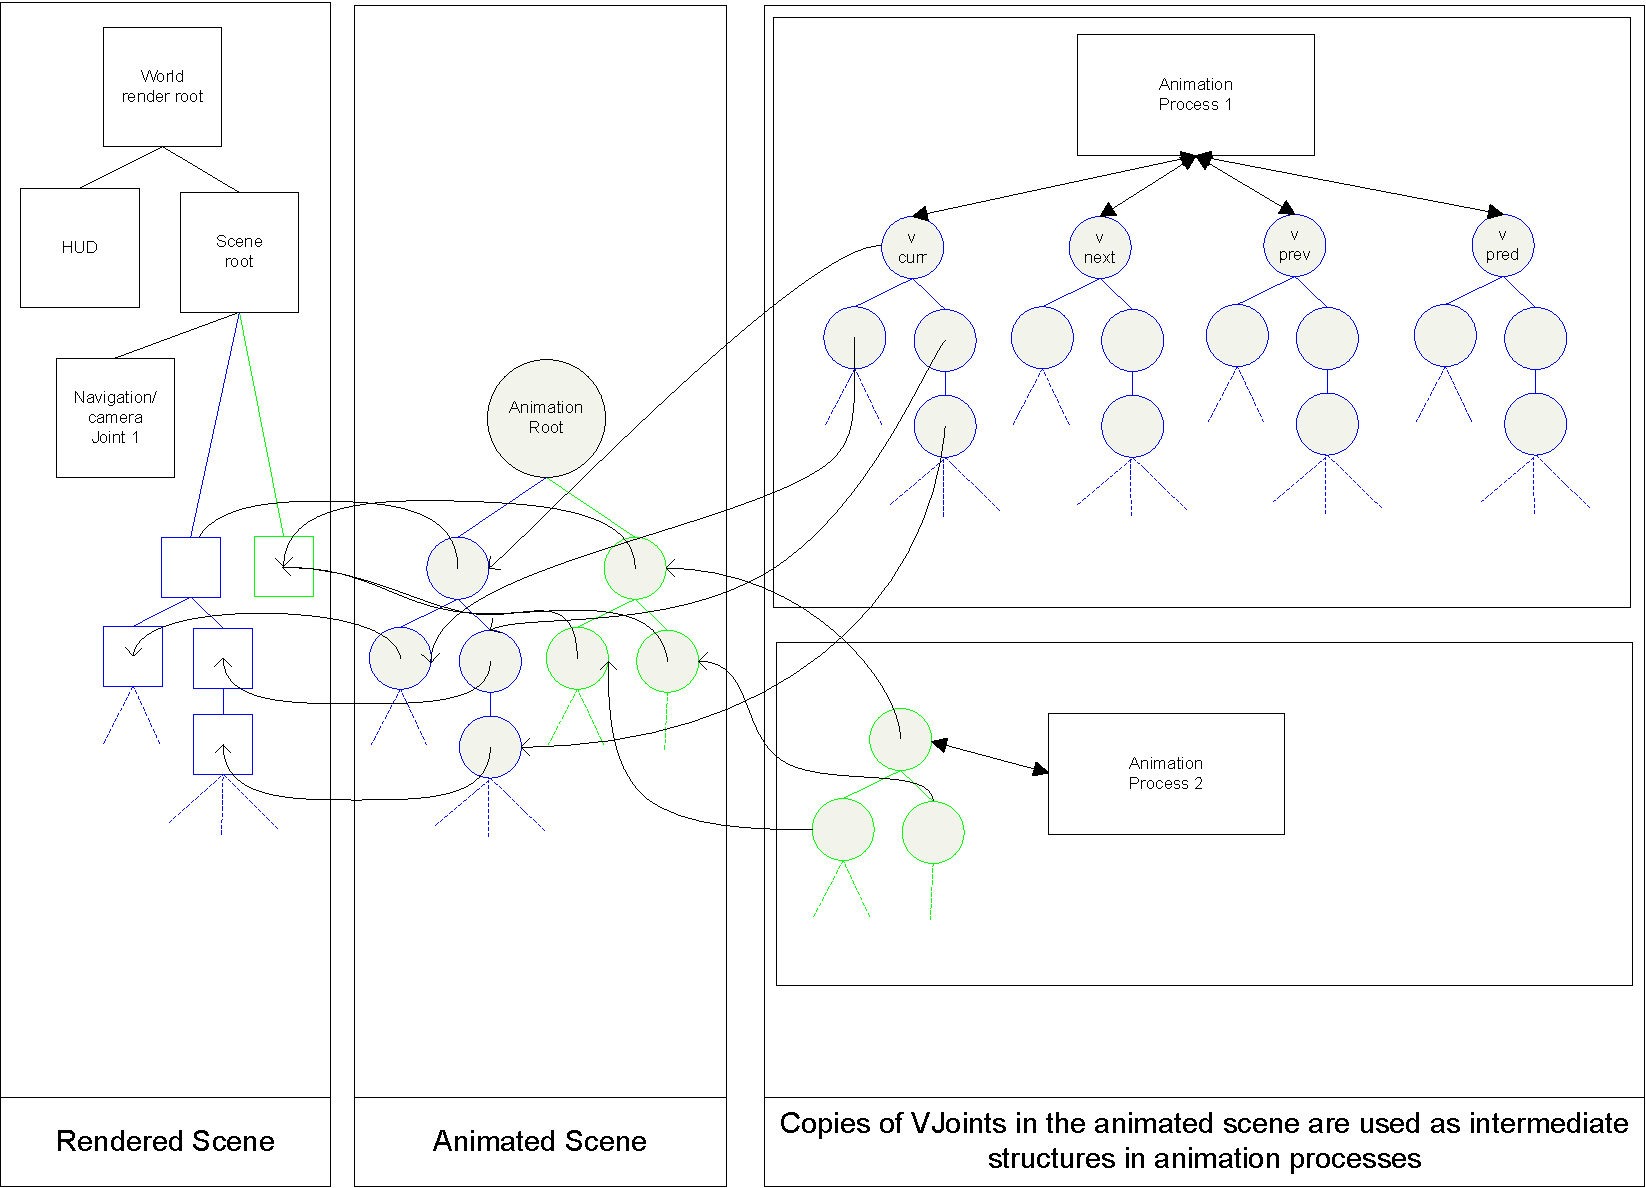
\includegraphics[width=13cm]{\hmianimationreportdir/typical_scenegraph}
\caption{\label{figuresg}Typical scenegraph layout}
\end{figure}

\begin{figure}
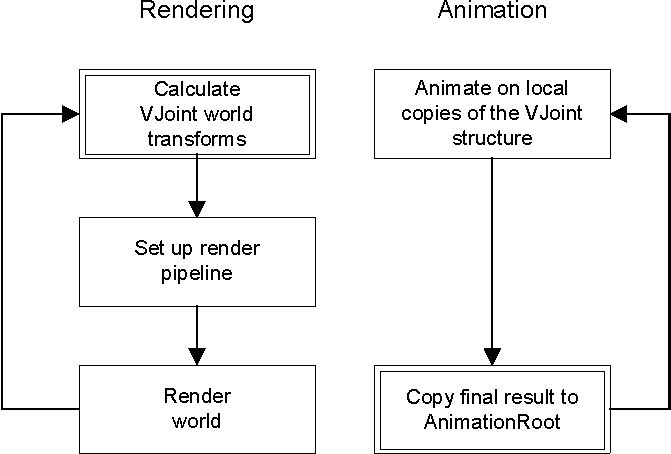
\includegraphics{\hmianimationreportdir/threads-crop}
\caption{\label{threads}Animation and rendering loops running in different threads. The processes with double lines are synchronized to each other.}
\end{figure}


 
\section{Procedural Animation}

\subsection{XML format}
...\\
Note that some symbols need to be XML encoded: $>$ as \&gt; , $<$ as \&lt; , \&\& as \&amp;\&amp; etc.
\subsubsection{JEP examples and custom macros}
Function of time ($0 \leq t \leq 1$) and float parameters (as constructed using \textless Parameter\textgreater).

\paragraph{If-statement}
\begin{verbatim}
if(<condition>,<expression_true>,<expression_false>)
\end{verbatim}
Evaluates the condition and executes 'expression\_true' if its true, expression\_false otherwise.

\paragraph{Random}
\begin{verbatim}rand()\end{verbatim}
Generates a random number between 0 and 1.

\paragraph{Hermite-spline}
\begin{verbatim}
hermite(time,v0,vn, p0,...,pn)
\end{verbatim}
Constructs a uniform Hermite spline, time distance between the points is 1.\\
time: time to execute the spline at, typically t*n to interpolate smoothly from p0 to pn as t ranges from 0 to 1.\\
v0:		speed at p0\\
vn:   speed at pn\\
pi:		position at i\\

\paragraph{TCB-spline}
\begin{verbatim}
tcbspline(time,v0,vn, p0,t0, pi,ti,tensi,conti,biasi,...,pn,tn)
\end{verbatim}
Constructs a non-uniform TCB spline.\\
time:time to execute the spline at $t0 \leq time \leq tn$\\
v0:  start speed\\
vn:  end speed\\
pi:  point i\\
ti:  time stamp i, $ti-1<ti<ti+1$\\
tensi: tensity i, $-1<tensity<1$, default = 0 \\
conti: continuity i, $-1<conti<1$, default = 0 \\
bias:  bias i, $-1<bias<1$, default = 0\\

 
%\ifx \hmigraphicsreportdir \undefinedmacro \def \hmigraphicsreportdir{.} \fi
\ifx \webserver \undefinedmacro \def \webserver{http://elckerlyc.sourceforge.net/javadoc/Hmi/} \fi
\chapter{The HmiGraphics packages}
The HmiGraphics and HmiAnimation packages constitute a framework for 3D graphics and animation, based upon Java and OpenGL.
This document describes the global structure of the various packages inside HmiGraphics and HmiAnimation.
The subdivision into HmiGraphics and HmiAnimation is largely based on the project structure used by build tools
like ant, Eclipse, and Netbeans. For an overview of the Hmi project structure, see \cite{hmiprojectstructure}

See the \href{\webserver}{javadoc}.



\section{Package overview}
The current contents of HmiGraphics and HmiAnimation is as follows:

\begin{itemize}
\item hmi.animation:
Deals with virtual objects, in particular animation of such objects. It defines a simple hierarchy of
virtual objects, by means of VJoints, primarily used for skeleton based animation of human avatars.
a virtual environment. Of course it is intended to be used in combination with the hmi.graphics packages,
but in principle it can be build and used independently.
\item hmi.graphics.collada:
Deals with reading (and to some extent writing) graphics files according to the Collada standard.
Apart from reading, it includes a sub package hmi.graphics.collada.scenegraph, for translating Collada descriptions into
hmi.graphics.scenegraph descriptions.
\item hmi.graphics.geometry:
Utility class, dealing with some purely geometric algorithms.
\item hmi.graphics.opengl:
Deals with actual rendering OpenGL based 3D graphics.
%It defines counterparts of some classes of the
%scenegraph package. For instance, we have the GLBasicMesh class which is sort of the hmi.graphics.opengl counterpart
%for the hmi.graphics.scenegraph GMesh class.
Although hmi.graphics.opengl is OpenGL based, it is still independent
of the  particular Java OpenGL binding or implementation. Currently there are two such OpenGL bindings: Jogl and LWJGL.
Each of these has its own package (hmi.graphics.jogl, hmi.graphics.lwjgl), and one of them must be used in combination with hmi.graphics.opengl.
hmi.graphics.opengl itself has a few sub packages:
\begin{itemize}
\item hmi.graphics.opengl.state: Contains classes for dealing with the OpenGL state management.
\item hmi.graphics.opengl.geometry: Defines a few utility classes for rendering simple geometry, like spheres, boxes, and lines.
\item hmi.graphics.opengl.scenegraph: Defines the translation from hmi.graphics.scengraph structures to hmi.graphics.opengl structures.
\end{itemize}

\item hmi.graphics.jogl and hmi.graphics.lwjgl are two packages that provide
actual OpenGL bindings, relying on native code in the form of windows dll files or Linux so files.
Both packages implement the GLRenderContext interface from hmi.graphics.opengl, and define
a simple Renderer.
Most of the JOGLContext and LWJGLContext code is generated, by means of a utility package hmi.graphics.gen.


\item hmi.graphics.scenegraph:
Defines scenegraph like structures for representing graphics data in a format independent of the external file format,
but also independent of the actual render technology being used.
\item hmi.graphics.util:
The usual package of our favorite ``utilities''.

\end{itemize}

Currently, there are a few more ``deprecated'' and/or temporary packages:
\begin{itemize}
\item hmi.graphics.colladatest:
Just for testing packages like collada, opengl, etcetera.
\item hmi.graphics.gen: used for generating files within  jogl and lwjgl implementations.
\item hmi.graphics.render
An attempt to create a platform neutral 3D renderer.
\end{itemize} 
%\section{Package dependencies}
We list the dependencies packages on our own hmi packages, as well as dependencies on non-standard
packages like Jogl or Ode.
Most packages depend on hmi.util and hmi.xml, and so we will not mention these for the sake of brevity.
\begin{itemize}
\item hmi.animation depends heavily on hmi.math. Otherwise it is quite independent, and it
 does explicitly \emph{not} depend on hmi.graphics packages,
nor on Jogl, LWJGL, or ODE.

\item hmi.graphics.scenegraph depends on hmi.math, hmi.graphics.geometry, and hmi.animation. It was designed to be independent of all other packages, in particular file format dependend packages like Collada, or render technology dependend packages like opengl, jogl, or lwjgl.

\item hmi.graphics.collada itself does not depend on other graphics packages. But it has a sub package hmi.graphics.collada.scenegraph that depends on hmi.graphics.scenegraph, hmi.graphics.collada, and hmi.math.

\item hmi.graphics.geometry does not depend on other packages

\item hmi.graphics.opengl depends on hmi.math, hmi.graphics.scenegraph, hmi.animation,
but \emph{not} on the Jogl or LWJGL.
The reference to hmi.animation is somewhat special:
the opengl package relies on VJoints for animation purposes. It is (only) here that the link between hmi.animation and
hmi.graphics is made.

\item hmi.graphics.jogl and hmi.graphics.lwjgl depend on hmi.graphics.opengl, as well as
on platform dependent dll files or so files, that reside inside the HmiGraphics/lib directory.
Inside the ant build files, the Jogl and LWJGL  dependencies can be denoted on
the ``dependencies'' line of \verb"build.properties", by means of the  \verb"Sun/jogl" or  \verb"LWJGL" tokens.
\item hmi.graphics.util, although small, combines various tools  and depends therefore on most other packages:
hmi.graphics.collada, hmi.graphics.opengl, and hmi.graphics.scenegraph.

\end{itemize}
%\section{The GLRenderContext: usage, implementation, and generation}
Rendering within the hmi.graphics package is OpenGL based. Several Java based implementations
and ``bindings'' for OpenGL exist. Currently, the most promising are Jogl (supported by Sun)
and LWJGL (very active community and some real commercial usage). Jogl is in a state of transition from a stable version based upon OpenGL 2.1 towards a new ``Jogl 2'' version that supports OpenGL 3.x. 
They all have much in common, since, basically, they are all just wrappers for the C functions from the OpenGL drivers.
At the same time, they differ enough so that one cannot serve as a ``drop in'' replacement for one of the others.
The answer to this unfortunate situation is (yet another) wrapper. (Fortunately, the wrapper is pretty straightforward and performance is not affected.)
Some of the differences between Jogl and LWJGL:
\begin{itemize}
\item Jogl represents the OpenGL context by means of an \emph{object} op type \verb"GL" that has a large number of methods, one for every relevant OpenGL function.  This is clearly the `object oriented'' style 
    and allows for more sophisticated handling of OpenGL by several processes concurrently. For instance, Jogl will
    (re-)acquire the OpenGL context  for every frame that is to be rendered. 
\item LWJGL on the other hand represents these OpenGL functions by means of \emph{static Java methods}, bundled in a few classes like \verb"GL11".
    The class names (\verb"GL11", \verb"GL12", ..., \verb"21") correspond to OpenGL versions $1.1, 1.2, ..., 2.1$.
    Each of them defines the methods for function introduced in that OpenGL version, which is nice if you want to keep track of the OpenGL version needed to run your application, but otherwise it's just an annoyance.  
\item In principle there would have been a one-to-one correspondence between the C functions for OpenGL and their Java counterparts, if Java would have dealt with pointers and arrays in the same style as within the C language. Such is not the case, and so each Java binding must somehow deal with function arguments like a pointer-to-float which is just the C representation of a float array parameter. There are some complications here, so there is no obvious solution, so, unavoidably,  Jogl and LWJGL have selected \emph{different} solutions.
    \begin{itemize}
     \item An ``array of floats'' is in C just a pointer to a float. That pointer points to the first element
     of the array, but by adding some ``offset'', it can point just as easily to some other starting point.
     \item An ``array of floats'' in Java can be represented as a Java float array, i.e. of type \verb"float[]".
     It can also be represented by means of a ``direct'' or ``indirect'' \verb"FloatBuffer" object. 
     \item Both Java float arrays and indirect \verb"FloatBuffers" are represented within the Java ``heap'', but direct \verb"FloatBuffers" are kept ``outside'' that heap. As a consequence, the Java native interface calls         can deal more efficiently with direct \verb"FloatBuffers" than with indirect buffers or float arrays. The flip side is that direct buffers are not automatically garbage collected, and although cpying large chunks of information from or to a direct buffer is ok, accessing individual buffer elements is not very efficient. (Basically, Java performs some checks when it passes information across the boundary of the Java virtual machine, for safety and security reasons). 
     \item Java float arrays have no means to represent ``offsets'' into an array the same way you can do this in C. But \verb"FloatBuffers" can represent such offsets by means of the current buffer position.
     \item Both Jogl and LWJGL use \verb"FloatBuffers" as the preferred way of representing C style float pointers. But Jogl also allows plain Java float arrays, as a convenience, whereas LWJGL suggest that you introduce a \verb"FloatBuffer" wrapper in such cases. When you do use an array in Jogl, you must also specify
         an ``offset'' in the form of a (long) integer, and as an ``extra'' argument for the Java method. 
    \end{itemize}
    
    
\end{itemize}
The \verb"GLRenderContext" interface from the hmi.graphics.opengl package (or more precisely, the \verb"GLBinding" sub-interface) has been introduced to get rid of the interface differences between Jogl and LWJGL. (It seems that the Jogl 2 interfaces introduce yet another variation, so we will capture that one as well).
The \verb"GLBinding" interface introduces a selection of the more useful OpenGL calls, and uses the more useful
 parameter conventions. So:
 \begin{itemize}
 \item Like Jogl, and unlike LWJGL, the \verb"GLBinding" interface represents the OpenGL conext by means of an Java object. The \verb"GLRenderContext" extends \verb"GLBinding", and adds a few render attributes, like the render ``pass''.
 \item There is one context, no annoying distictions between OpenGL versions.
 \item \verb"FloatBuffers" are preferred, but for a few cases float arrays are allowed as convenience method, but without the superfluous integer offset from Jogl. (When you really  want offsets, you want to use \verb"FloatBuffers" anyway)
 \end{itemize}
 
 \subsection{Generating the Java bindings}
 From the section above it should be clear that we have a number of Java classes and interfaces that need to be ``in sync'' so to say. These are:
 \begin{enumerate}
 \item \verb"GLRenderContext" and \verb"GLBinding.java" from hmi.graphics.opengl
 \item \verb"JOGLContext" from hmi.graphics.jogl
 \item \verb"LWJGLContext" from hmi.graphics.lwjgl
 \end{enumerate} 
 Rather than manually updating each of these files, they are being \emph{generated} from a common definitions file called \verb"GLF.def", located in hmi.graphics.opengl, plus a few short binding-specific header files. The \verb"GLF.def" files contains templates from which the three files above can be generated. The \verb"GLBinding.header", \verb"JOGLContext.header", and \verb"LWJGLContext.header" deal with the few things that could not be dealt with in a generic way.
 
 To be concrete:
 \begin{enumerate}
 \item \verb"GLBinding.java" is generated by running \verb"GenGLBinding" from the hmi.graphics.gen package.
 (\verb"GLRenderContext" simply extends \verb"GLBinding", so it us updated implicitly)
 \item \verb"JOGLContext" is generated by running \verb"GenJOGLContext" from hmi.graphics.gen
 \item \verb"LWJGLLContext" is generated by running \verb"GenLWJGLContext" from hmi.graphics.gen
 \end{enumerate}
 
 
  The format for the \verb"GLF.def" file is as follows:
  \begin{itemize}
  \item A line like :\\
  \verb"GL11  public void glClear(int mask);"\\
  denotes a simple OpenGL function \verb"glClear" with one int-typed argument called \verb"mask". 
  It is prefixed by \verb"GL11" to denote that it is an OpenGL 1.1 function. ( Jogl  will ignore this,
  but  LWJGL  needs it.)
  \item The two lines:\\
  \verb"GL11  public void glGetFloatv(int pname, FloatBuffer params);"
  \verb"GL11  public void glGetFloatv(int pname, float[] params);"\\
  denote two variations of the OpenGL function \verb"glGetFloatv", one with a \verb"FloatBuffer",
  one with a Java float array. Note that we have no Jogl-style array offset.
  For Jogl, the translation in JOGLContext.java becomes:\\
  \verb"public final void glGetFloatv(int pname, FloatBuffer params) "\\
  \verb"  { gl.glGetFloatv(pname, params); }"\\
  \verb"public final void glGetFloatv(int pname, float[] params) "\\
  \verb"  { gl.glGetFloatv(pname, params, 0); }"\\
  Whereas for LWJGL, we have inside LWJGLContext.java:\\
  \verb"public final void glGetFloatv(int pname, FloatBuffer params)  "\\
  \verb"  { GL11.glGetFloat(pname, params); }"\\
  \verb"public final void glGetFloatv(int pname, float[] params)  "\\
  \verb"  { GL11.glGetFloat(pname, FloatBuffer.wrap(params));}"\\
  
  \item Finally, we sometimes need some "hack" in cases like this line in \verb"GLF.def":\\
  \verb"GL11  public void glDrawElements"\\
  \verb"    (int mode, int bufcount, int buftype, IntBuffer indices);"\\
  For Jogl, this translated in straightforward manner:\\
  \verb"public final void glDrawElements"\\
  \verb"    (int mode, int bufcount, int buftype, IntBuffer indices)"\\
   \verb"   { gl.glDrawElements(mode, bufcount, buftype, indices); }"\\
   But for LWJGL, the fact that we use an \verb"IntBuffer" argument is used to infer the buftype and bufcount
   arguments. So the translation becomes:\\
   \verb" public final void glDrawElements"\\
   \verb"   (int mode, int bufcount, int buftype, IntBuffer indices) "\\
   \verb"   { GL11.glDrawElements(mode, indices); }"\\
  \end{itemize}
  
  This works only because of a "hack": the two parameter names \verb"bufcount" and \verb"buftype"
  are recognized as such when used in a parameterlist where also some buffer is used,
  and the LWJGL translation will omit them for the LWJGL translation. 
\section{Skeleton Structures for avatars}
An avatar that is to be used for (bodily) animation must
posses a \emph{skeleton} or \emph{bones} structure.
By this we do not mean a physical model or a visualization of
a real skeleton, but rather a structure consisting \emph{joints} and
\emph{segments} or \emph{bones} that is to be used for the purpose of animation.
See the picture in \autoref{figure:skeleton} for an example skeleton.
%\vspace{ex}
A skeleton consists of \emph{joints}, like the Pelvis or Spine nodes in the picture,
connected by means of \emph{segments} (or ``\emph{bones}''), shown here by means
of arrows connecting the joints. It will be clear that a skeleton is a rooted tree.
(For the example skeleton, the root node is the Pelvis node)




\begin{figure}

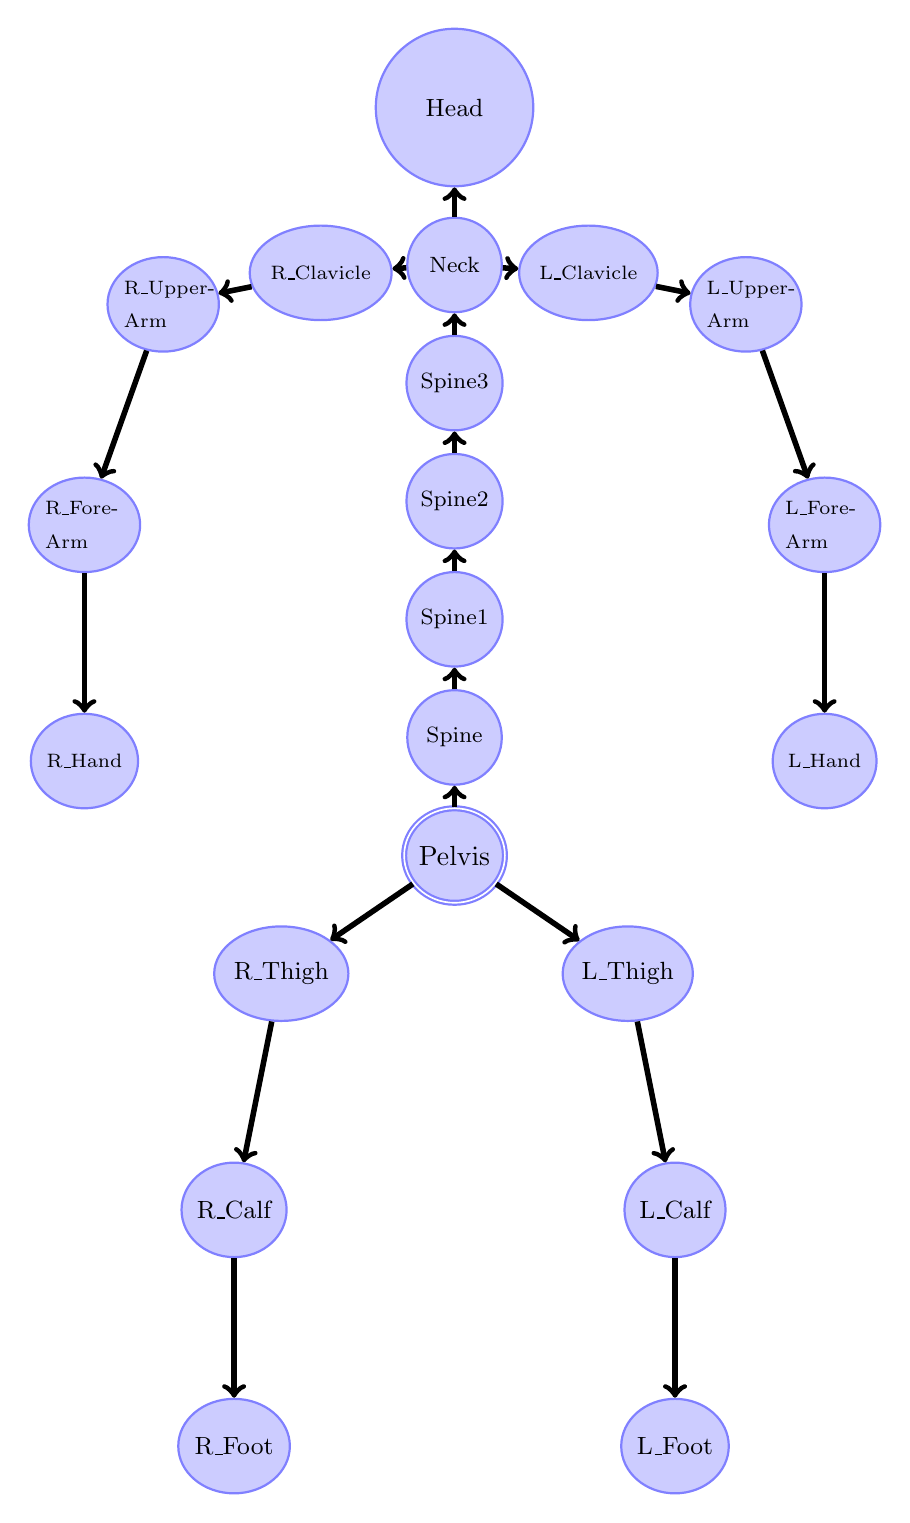
\begin{tikzpicture}
  [joint/.style={shape=ellipse,draw=blue!50,fill=blue!20, thick,
         inner sep=0pt, minimum width=12mm, minimum height=12mm}
  ]

 \path
   (0, 0) node (pelvis)            [joint, double] {Pelvis}
   {[current point is local] % start upper body branch, from pelvis
      ++(0, 1.5)   node (spine)      [joint]         {\footnotesize Spine}
      ++(0, 1.5)   node (spine1)     [joint]         {\footnotesize Spine1}
      ++(0, 1.5)   node (spine2)     [joint]         {\footnotesize Spine2}
      ++(0, 1.5)   node (spine3)     [joint]         {\footnotesize Spine3}
      ++(0, 1.5)   node (neck)       [joint]         {\footnotesize Neck}
      {[current point is local] % start head branch, from neck
         ++(0, 2.0) node (head)       [joint, minimum size=20mm] {\small Head}
      }
      {[current point is local] % start left arm branch, from neck
         ++(1.7, -0.1)   node (lclavicle)  [joint] {\scriptsize L\_Clavicle}
         ++(2.0, -0.4)   node (lupperarm)  [joint, text width=10mm] {\scriptsize L\_Upper\-Arm}
         ++(1.0, -2.8)   node (lforearm)   [joint,  text width=10mm] {\scriptsize L\_Fore\-Arm}
         ++(0.0, -3.0)   node (lhand)      [joint] {\scriptsize L\_Hand}
      }
      {[current point is local] % start right arm branch, from neck
         ++(-1.7, -0.1)  node (rclavicle)  [joint] {\scriptsize R\_Clavicle}
         ++(-2.0, -0.4)  node (rupperarm)  [joint, text width=10mm] {\scriptsize R\_Upper\-Arm}
         ++(-1.0, -2.8)  node (rforearm)   [joint,  text width=10mm] {\scriptsize R\_Fore\-Arm}
         ++(0.0,  -3.0)    node (rhand)    [joint] {\scriptsize R\_Hand}
      }
   }
      {[current point is local] % start left leg branch, from pelvis
         ++(2.2, -1.5) node (lthigh)  [joint] {\small L\_Thigh}
         ++(0.6, -3) node (lcalf)   [joint] {\small L\_Calf}
         ++(0, -3)   node (lfoot)   [joint] {\small L\_Foot}
      }
      {[current point is local] % start right leg branch, from pelvis
         ++(-2.2, -1.5) node (rthigh)  [joint] {\small R\_Thigh}
         ++(-0.6, -3) node (rcalf)   [joint] {\small R\_Calf}
         ++(0, -3)    node (rfoot)   [joint] {\small R\_Foot}
      }
   ;
   \begin{scope}[line width=2pt]
   \draw [->] (pelvis) -- (spine);
   \draw [->] (spine) -- (spine1);
   \draw [->] (spine1) -- (spine2);
   \draw [->] (spine2) -- (spine3);
   \draw [->] (spine3) -- (neck);
   \draw [->] (neck) -- (head);
   \draw [->] (neck) -- (lclavicle);
   \draw [->] (lclavicle) -- (lupperarm);
   \draw [->] (lupperarm) -- (lforearm);
   \draw [->] (lforearm) -- (lhand);
   \draw [->] (neck) -- (rclavicle);
   \draw [->] (rclavicle) -- (rupperarm);
   \draw [->] (rupperarm) -- (rforearm);
   \draw [->] (rforearm) -- (rhand);
   \draw [->] (pelvis) -- (lthigh);
   \draw [->] (lthigh) -- (lcalf);
   \draw [->] (lcalf) -- (lfoot);
   \draw [->] (pelvis) -- (rthigh);
   \draw [->] (rthigh) -- (rcalf);
   \draw [->] (rcalf) -- (rfoot);
   \end{scope}

\end{tikzpicture}
\caption{Example of a skeleton structure}\label{figure:skeleton}
\end{figure} 

\def\Alocal{\mathstrut^L\!A}


%\[
%{}^{14}_{2}\mathbf{C}^{5+}_{2} \quad
%\prescript{14}{2}{\mathbf{C}}^{5+}_{2} \quad
%\prescript{4}{12}{\mathbf{C}}^{5+}_{2} \quad
%\prescript{14}{}{\mathbf{C}}^{5+}_{2} \quad
%\prescript{}{2}{\mathbf{C}}^{5+}_{2}
%\]


\subsection{Affine and linear transforms}
Within this chapter by \emph{linear} transform we mean an ordinary linear mapping for 3D space, represented
by a $3\times 3$ matrix $M$.
A \emph{translation} $T$ is defined by a 3D translation vector $t$.
When we want to make this vector it explicit, we write $T_t$ for a translation operation.
As is well known, a translation operation $T$ is not linear, so cannot be represented by a $3\times 3$ matrix.
We often need the combination $A$ of a linear transform $M$ followed by a translation $T$, so $A=T\circ M = T\,M$.
Such a combination is called an \emph{affine} transform.
The combination in the reverse order, i.e. $M\,T = M\, T_t$ is also affine, since it is equivalent
to the affine transform $A = T_{t'} \, M$, where $t'=M(t)$.
As a consequence, a composition of affine transforms $A_0$ and $A_1$ is itself also affine:
%
\begin{gather}\label{affinecomposition}
A_0A_1 = T_{t_0}\,M_0\, T_{t_1}\, M_1 = T_{t_0}\,T_{M_0(t_1)}\,  M_0 \,M_1 =
T_{t'}M',\\
\text{where } t' = t_0 + M_0(t_1) \text{ and } M' = M_0\, M_1.\notag
\end{gather}
%

\noindent
A (non-degenerate) linear transformation can be an \emph{orthogonal} matrix $Q$
which for 3D spaces is either a pure \emph{rotation} $R$, or else a rotation combined with a \emph{reflection}.
(In the latter case it can represented, for instance, as $Q=R\,N$, where $R$ is a pure rotation,
and where $N$ is a reflection. For instance, one may choose $N$ to be $-I$.
Another important class of linear transforms is that of \emph{scaling}.
In the simplest case, a scaling matrix $S$ is just the ($3\times 3$) identity matrix multiplied
with a \emph{uniform scaling} factor $s$. A more complex case is when $S$ is a diagonal matrix
with three different scaling factors $s_x$, $s_y$, and $s_z$ on the diagonal, which represents axis-aligned
\emph{non-uniform scaling}. In the most complicated case, a scaling matrix $S$ is
not even diagonal, but it would be diagonal in some rotated coordinate system.
So it represents \emph{non-unform scaling along rotated axes}, a situation sometimes called \emph{skewing}.
An important result here is that by means of so  called \emph{polar decomposition}
any (non-degenerate) 3D matrix $M$ can be decomposed as $M=Q\, S$,
where $Q$ is orthogonal, and where $S$ is a scaling matrix. A nice property of polar decomposition
is that $Q$ is not just \emph{any} orthogonal matrix, but that among all orthogonal matrices it is the one
that is \emph{closest} to $M$. We conclude that, for our purpose, we may assume that
any linear 3D matrix $M$ has the form $R\,S$ where $R$ is a pure rotation and where $S$ is a scaling matrix,
possibly combined with a reflection operation.
Our affine transforms $A$ are therefore of the form $T\,R\,S$. Although $A$ is not a 3D linear transform
it \emph{can} be represented by a $4\times 4$ \emph{homogeneous} transform matrix.
So $A$ has a matrix with the $3\times 3$ matrix for $R\,S$ in the upper left part, the translation vector
$t$ for the translation $T$ in the rightmost column, and a
 bottom row of the form $(0,\;0,\;0,\; 1)$.



\subsection{Skeleton transforms}
\label{sect:skeletontransforms}

The main use of skeletons is that they organize a collection of transforms, one transform for every skeleton joint $J_i$.
Note: skeleton joints are sometimes called ``bones''. This terminology is slightly confusing since for others ``bones'' refer to
the skeleton segments in between the joints.


For joint transformations we must distinguish between a \emph{local transforms} $D_i$ versus the \emph{global transforms} $A_i$
associated with each joint $J_i$.
The local transform represents the transform caused by that single joint alone.
The global transform $A_i$, is the combined effect of all joints
on the path from the skeleton root up to and including the joint itself.
For instance, for the joint called L\_Forearm in the example skeleton,
the global matrix $A_\text{L\_Forearm}$ represent the rotations and translations
from the Pelvis joint, the various Spine joints, the Neck joint, the
L\_Clavicle joint, L\_UpperArm joint, and finally the L\_ForeArm joint itself.

The \emph{local transform} $D_i$  for a joint represents just the rotation $R_i$ (and possibly scaling $S_i$)
introduced by that joint alone, together with the translation that represents the vector $t$ from the parent
of that joint to the joint itself.
For instance, for the L\_ForeArm joint the local translation is represented by the vector from L\_UpperArm to L\_ForeArm.
Note that each $D_i$ is an affine transform.


 The idea of a skeleton is that joint transformations are build up hierarchically, following the tree
 structure of the skeleton. So, when some joint $J_i$ has joint $J_p$ as its parent,
 then $A_i = A_p \, D_i$, where $A_p$ is the transform associated with $J_p$,
 and where $D_i$ is the \emph{local} transform associated with joint $J_i$.
 For the special case of the root joint $J_0$, there is no parent, and we assume that in this case the
 transform $A_0$ is simply equal to the local transform $D_0$.
 For long chains of joint, we can thus factorize the transform $A$ of the end of the chain into
 the local transforms of the joints on the chain. For instance, for the example skeleton
 we can calculate the affine matrix of, say, the neck joint as follows:
 %
  \begin{equation}
  A_\textit{Neck} = D_\textit{Pelvis} \: D_\textit{Spine} \: D_\textit{Spine1} \: D_\textit{Spine2} \: D_\textit{Spine3} \:D_\textit{Neck}
  \end{equation}
%

\begin{figure}

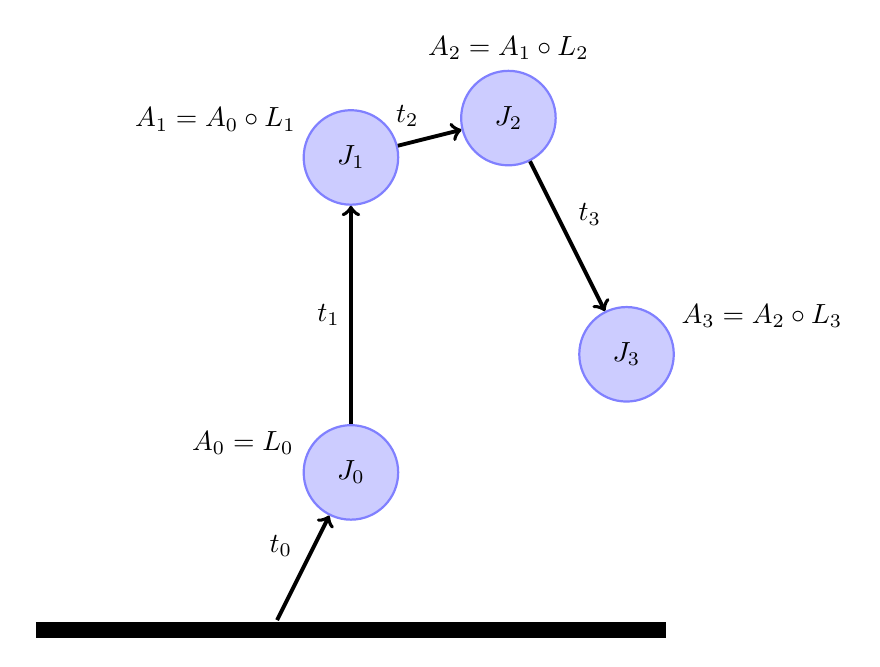
\begin{tikzpicture}
  [joint/.style={shape=ellipse,draw=blue!50,fill=blue!20, thick,
         inner sep=0pt, minimum width=12mm, minimum height=12mm},
  auto
  ]
   \begin{scope}[line width=6pt]

  \draw (-4,0) -- (4,0);
   \end{scope}
  \node (origin) [minimum size = 0] at(-1, 0) {  };
 \path
   (0, 2) node (j0)        [joint, label=170:{$A_0=L_0$}] {$J_0$}
  ++(0, 4)   node (j1)   [joint, label=160:{$A_1=A_0\circ L_1$}]         {$J_1$}
  ++(2, 0.5)   node (j2)    [joint, label=90:{$A_2=A_1\circ L_2$}]         {$J_2$}
  ++(1.5, -3)   node (j3)     [joint, label=20:{$A_3=A_2\circ L_3$}]         {$J_3$}

   ;
   \begin{scope}[line width=1.4pt]
   \draw [->] (origin) to node{$t_0$} (j0);
   \draw [->] (j0) to node{$t_1$}(j1);
   \draw [->] (j1) to node{$t_2$}(j2);
   \draw [->] (j2) to node{$t_3$}(j3);
   \end{scope}

\end{tikzpicture}
\caption{Part of a skeleton, with Translations $t_i$, Local Transforms $D_i$, and global transforms $A_i$}\label{figure:skeletonfragment}
\end{figure} 
For the smaller scale example from \autoref{figure:skeletonfragment}, we have:
%
\begin{equation}\label{eq:a3}
 A_3 = A_2\: D_3 = A_1 \: D_2\: D_3 = A_0\: D_1\:D_2\:D_3 = D_0\: D_1\:D_2\:D_3.
 \end{equation}
%
% WinEDT bug triggered by this line??:
%
\begin{figure}

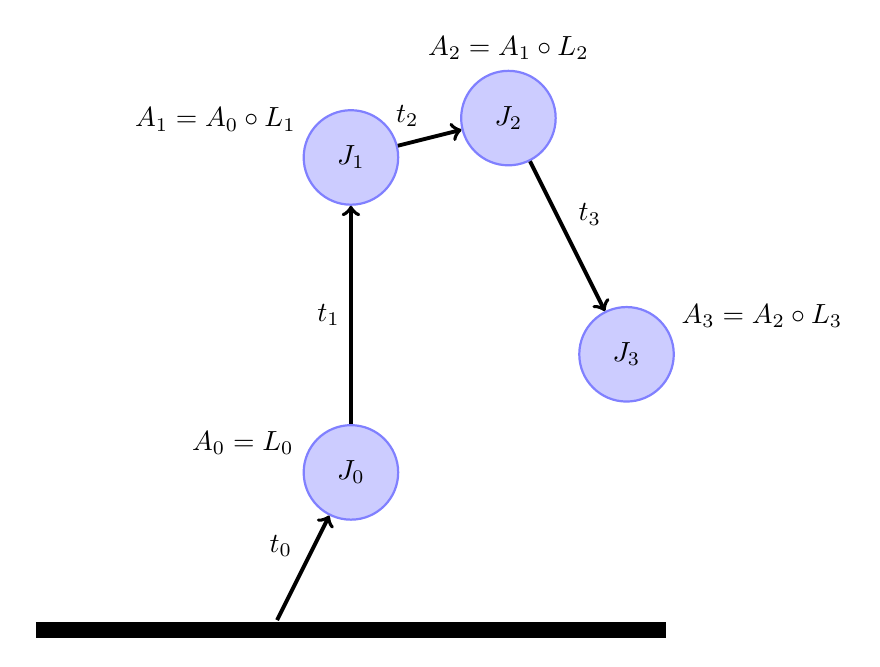
\begin{tikzpicture}
  [joint/.style={shape=ellipse,draw=blue!50,fill=blue!20, thick,
         inner sep=0pt, minimum width=12mm, minimum height=12mm},
  auto
  ]
   \begin{scope}[line width=6pt]

  \draw (-4,0) -- (4,0);
   \end{scope}
  \node (origin) [minimum size = 0] at(-1, 0) {  };
 \path
   (0, 2) node (j0)        [joint, label=170:{$A_0=L_0$}] {$J_0$}
  ++(0, 4)   node (j1)   [joint, label=160:{$A_1=A_0\circ L_1$}]         {$J_1$}
  ++(2, 0.5)   node (j2)    [joint, label=90:{$A_2=A_1\circ L_2$}]         {$J_2$}
  ++(1.5, -3)   node (j3)     [joint, label=20:{$A_3=A_2\circ L_3$}]         {$J_3$}

   ;
   \begin{scope}[line width=1.4pt]
   \draw [->] (origin) to node{$t_0$} (j0);
   \draw [->] (j0) to node{$t_1$}(j1);
   \draw [->] (j1) to node{$t_2$}(j2);
   \draw [->] (j2) to node{$t_3$}(j3);
   \end{scope}

\end{tikzpicture}
\caption{Part of a skeleton, with Translations $t_i$, Local Transforms $D_i$, and global transforms $A_i$}\label{figure:skeletonfragment}
\end{figure} 


%
We can decompose each local affine transform $D_i$ into a linear transform $L_i$ followed by
a translation $T_{t_i}$, thus: $D_i = T_{t_i}\: L_i$.
Using \eqref{affinecomposition} we can rearrange equation \eqref{eq:a3}.
%
\begin{gather}
A_3 = T_t \: L\\
 \text{where } t = t_0 + L_0(t_1) + L_0\,L_1(t_2) + L_0\,L_1\,L_2(t_3)\notag\\
 \text{and where } L= L_0\,L_1\,L_2\,L_3.\notag
\end{gather}
%
So the net effect of a ``chain'' of local affine transforms, from skeleton root up to some skeleton joint,
is equivalent to a single affine transform for that joint, which we have introduced before: it is the
\emph{global} transform for a joint.

\subsection{Weight blending}\label{sect:weightblending}



Skeletons can be controlled and used by animation software; in those cases, we are only concerned
with the local and global joint transforms. But skeletons are also used as an interface between
animation engines and graphics rendering engines.
In this case, the skeleton transforms are used
to transform geometry that is used for rendering objects, in particular for rendering human avatars.
The general idea is that there are one or more \emph{meshes}, each consisting of many polygons,
that model the  geometric shape of body parts.
There are two fundamentally different ways of doing this.
One rather simple approach is to cut an animated object into parts, each of which is then animated independently,
under the control of a single joint, dedicated to that part. For example, the ``blue guy'' avatar
uses this approach, and uses separate meshes for limbs and other body part.
The geometry associated with the elbow region of the body  is transformed exclusively
by the global affine transform for the elbow joint.
One of the advantages of this simple approach is that all mesh vertices inside a single body part
are transformed by the same affine matrix; a situation that suits the classical render pipeline
of graphics hardware, as well as the OpenGL and DirectX interfaces for that hardware.
 Simple or not, an unavoidable problem with this approach is that an avatar body as a whole
 shows seams at places where different body parts connect.

 An improved form of animating objects like human avatars is to use only \emph{one seamless mesh},
 and to use the skeleton transforms to deform by the following process:
 Each mesh vertex $v$ is transformed under the influence of one or more joints $J_{i_0}, \ldots, J_{i_n}$,
 with \emph{weights} $w_{i_0}, \ldots, w_{i_n}$ determining the relative influence of each joint.
 The exact set of joints and weights is unique for every individual vertex. Of course, one expects
 that most vertices will be controlled by a fairly low number of joints, typically one or two, and almost always less than four,
 all located in the neighborhood of the vertex. We would like to write down the transformation for some vertex $v$.
 We denote the global transform for joint $J_i$ by $A_i$ and, for simplicity, we assume that we have some vertex $v$
 that is influenced by joints $J_0, \ldots J_n$.
 The combined transform for $v$ using weight blending is defined as follows
%
\begin{equation}\label{eq:weightblending-simple}
 v' = \sum_{i=0}^{n} w_i\, A_i(v)
\end{equation}

\subsection{Bind poses}
Weight blending is an adequate animation method, but it requires both a suitable mesh as well
as a skeleton that ``fits'' into the mesh. A problem here is that designers of meshes and designers
of skeleton-based animations have slightly conflicting interests:
An animation system would prefer a skeleton that is in some well defined neutral pose
when all joint rotations are set to identity transforms. In that case all affine transforms
reduce to mere translations. The HAnim standard for skeleton based animation, for instance,
requires that in this situation the human avatar has a well defined pose where the body is upright,
arms are pointing downwards, fingers are pointing downwards, the thumbs have a $45^\circ$ degree orientation
relative to the fingers, etcetera.
The advantage of such a neutral pose is that an animation engine can put the avatar in some pose by setting well defined
rotations within joints.

Designers of nice looking avatar meshes though, prefer a \emph{different} pose, usually with the arms
horizontally stretched, also known as the ``T-pose''. The main reason here is that graphics designers
need to work on detailed graphic detail, and some areas like arm pits are difficult to reach and problematic when
the avatar is in the HAnim neutral pose, rather than the T-pose.
There are some variations of this ``T-pose'', for instance with the arms in a straight line but in a slightly lowered
position.

The result is that meshes and skeleton structures usually do \emph{not} automatically ``match'', and we need some
process called ``binding'' the mesh to the skeleton. One of the steps in the binding process is
that the skeleton, starting initially in its neutral pose, is put into ``bind pose'', by applying suitable
rotations for its joints. For example, for our HAnim style skeleton, the bind pose for a T-shape avatar
would include a $90^\circ$ rotation for the shoulder joints, in order to get the arms into the T-pose.
Other joints, for instance for arms and fingers, will likely have also non-identity
rotations in the bind pose, although angles will not be as large as the $90^\circ$ degree rotations for the shoulders.
In other situations for instance in the case of exporting a virtual character from a tool like 3DSMax, the
tool itself might use rather complicated transformations internally for binding a mesh to a skeleton.
Unfortunately such more or less ad hoc bind poses show up when you export the mesh to some external format,
for instance in the FBX format or the Collada format
The message here is that,even if you are willing to design your character in HAnim pose,
you still might have to deal with non-trivial bind poses.

After putting a skeleton in bind pose,
the next step in the bind process is to assign blend weights to the vertices in the mesh.
We won't discuss this (complicated) step here, and assume that you have used some tools to do this.
For instance,  most 3D modeling tools have a process called ``weight painting'' that allow you to establish blend weights
in a more or less intuitive way. In practice, assigning blend weight is a trial and error process.

We continue with the problems for our animation engine,
caused by the difference in the neutral skeleton pose and bind pose.
Say we would like our avatar to be in our neutral pose when all joint rotations
are set to identity.
It is clear that we must adapt our equation \ref{eq:weightblending-simple}
for weight blending.
Somehow, we must take into account the joint transforms that were used to
get the skeleton into the correct bind pose. Let's assume that we know the values for (global) affine joint matrices
in the bind pose, and let's call these matrices the \emph{bind matrices} $B_i$.
The intuitive idea is that we can use the \emph{inverse} bind matrices $B_i^{-1}$ to bring our mesh
back into the neutral pose, and from that neutral pose, we bring it into the desired pose for some animation
specified by (global) joint matrices $A_i$.
This suggest our improved weight blending equation:
%
\begin{equation}\label{eq:weightblending}
 v' = \sum_{i=0}^{n} w_i\, A_i\,B_i^{-1}(v)
\end{equation}
%
One way of seeing that this must be the ``correct'' equation is to put the avatar in its bind pose again,
 by choosing joint transformations $A_i$ equal to the bind matrices $B_i$:
 for in that case the $A_i$ and $B_i^{-1}$ matrices cancel,
and we have that for all vertices $v' = v$. Which is correct, since the mesh without transforms applied is,
by definition, in the bind pose.

Since bind matrices are \emph{fixed}, one might think that you can get rid of the inverse bind matrices
in \autoref{eq:weightblending} by applying these inverse bind matrices just once to the mesh, and
store the resulting transformed mesh, which would now be in the (by animators) desired neutral pose.

\noindent
This idea \emph{would} work if every vertex $v$ would be associated with just a single joint, so for the simple
model from section \ref{sect:weightblending}, one could transform the various body parts by applying
the unique $B_i^{-1}$ for that part. (Note that for the rather special case where the bind pose
is actual the same as the neutral pose, the bind matrices would reduce to  pure translations of the
form $T(C_i)$, where $C_i$ is the center position of joint $J_i$. So in this particular case,
applying $B_i^{-1}$ boils down to a ``shifting back to the origin'' operation for the various body parts.)

\noindent
Unfortunately, the idea breaks down when more than one joint influences some vertex $v$.
Why? let's try. So we store, in an offline process, the mesh transformed into its neutral pose.
The result is that we have transformed vertex $v$ into a vertex $v'$ defined by:
$ v' = \sum_{i=0}^{n} w_i\, B_i^{-1}(v)$.
If we now apply \autoref{eq:weightblending-simple}, where we replace $v$ by our ``corrected'' vertices $v'$,
then we get the following vertex $v''$ as the result of applying a pose defined by joint matrices $A_i$:
%
\begin{equation}\label{eq:weightblending-problem}
 v'' = \sum_{i=0}^{n} w_i\, A_i(v') = \sum_{i=0}^{n} w_i\, A_i(\sum_{j=0}^{n} w_j\, B_j^{-1}(v))
\end{equation}
%
This last equation \ref{eq:weightblending-problem} clearly does not yield the
same results as equation \ref{eq:weightblending}.
Fortunately, we can modify and simplify bind matrices if we are willing to adapt transformation matrices
$A_i$ from animations. We discuss this below.

% second time , but otherwise WinEdt will have problems:

\begin{figure}

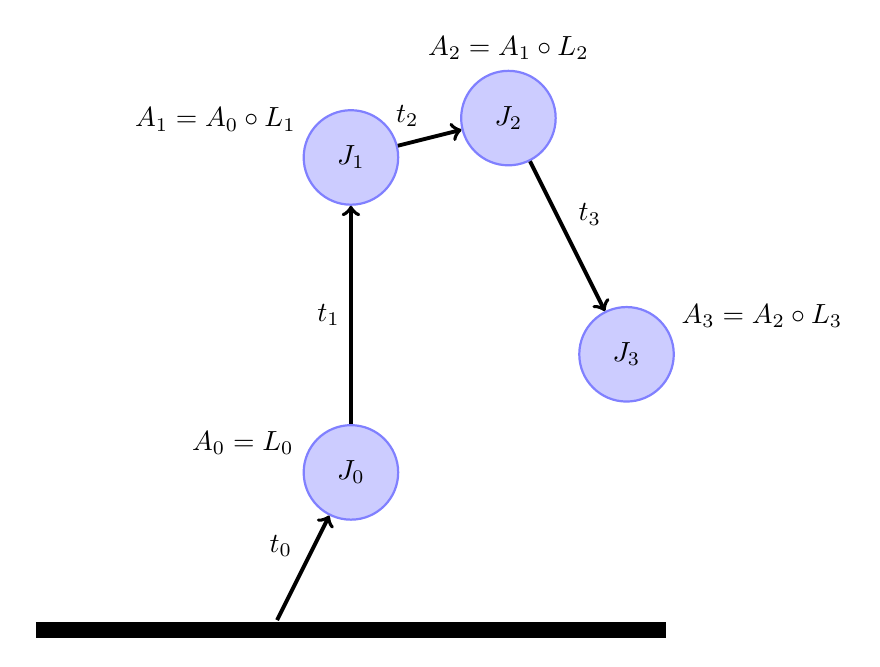
\begin{tikzpicture}
  [joint/.style={shape=ellipse,draw=blue!50,fill=blue!20, thick,
         inner sep=0pt, minimum width=12mm, minimum height=12mm},
  auto
  ]
   \begin{scope}[line width=6pt]

  \draw (-4,0) -- (4,0);
   \end{scope}
  \node (origin) [minimum size = 0] at(-1, 0) {  };
 \path
   (0, 2) node (j0)        [joint, label=170:{$A_0=L_0$}] {$J_0$}
  ++(0, 4)   node (j1)   [joint, label=160:{$A_1=A_0\circ L_1$}]         {$J_1$}
  ++(2, 0.5)   node (j2)    [joint, label=90:{$A_2=A_1\circ L_2$}]         {$J_2$}
  ++(1.5, -3)   node (j3)     [joint, label=20:{$A_3=A_2\circ L_3$}]         {$J_3$}

   ;
   \begin{scope}[line width=1.4pt]
   \draw [->] (origin) to node{$t_0$} (j0);
   \draw [->] (j0) to node{$t_1$}(j1);
   \draw [->] (j1) to node{$t_2$}(j2);
   \draw [->] (j2) to node{$t_3$}(j3);
   \end{scope}

\end{tikzpicture}
\caption{Part of a skeleton, with Translations $t_i$, Local Transforms $D_i$, and global transforms $A_i$}\label{figure:skeletonfragment}
\end{figure} 

\subsubsection{Adjusting bind matrices}

We have seen the generic weight blending equation \ref{eq:weightblending} above.
There are various situations where we would like to modify the (inverse) bind matrices $B_i^{-1}$,
thereby redefining the ``neutral pose'' for a character.
One reason could be that the neutral pose as defined by some 3D modeling tool is inconvenient.
For instance, the neutral position for a Collada export from 3DSMax defines a rather strange looking ``neutral'' position.
Moreover, in such modeling tools the character mesh is often aligned with the Z-axis, (called the ``up-axis'') and for our animation engine
we prefer a world where the Y-axis is the ``up-axis''. A final reason would be
that we want to switch to a \emph{new} neutral position like the one defined by the HAnim standard.
In all such cases, three things have to happen:
\begin{enumerate}
\item The \emph{(inverse) bind matrices} must be changed. This can be done by multiplying $B_i^{-1}$
by matrices $V_i$ that must be chosen in a suitable way for each of the situations mentioned above.
\item The local \emph{rotations} for every joint to be used for various poses in animations must be adapted accordingly.
This step is necessary only when existing animation data that was created for the ``old'' bind matrices.
When new animation data has to be produced it might be much more convenient to work immediately with
the ``new'' bind matrices. For instance, if we switch bind matrices that are suitable for HAnim then
new animation data should use the HAnim pose as ``neutral'' pose. On the other hand, existing animation data,
for instance, data exported from the 3D modeling tool, will be based upon the ``original'' bind matrices, and so
we have to convert the rotations from that data.
\item The local \emph{translations} for every joint must be adapted to the new bind matrix.
This can be done once, since translations and (modified) bind matrices are not changed by animation data.
The only exception here that we allow is the ``humanoid root translation'' $t_0$, for the root joint $J_0$:
this translation is sometimes modified in animations.
\end{enumerate}
%
We discuss here first the generic case, where we multiply $B_i^{-1}$ by arbitrary $V_i$.
We assume here that $V_i$ is just a rotation, and contains no translation.
That means that we replace an inverse bind matrix $B_i^{-1} = U_i^{-1}\,T_{-C_i}$
by ${B'}_i^{-1} = V_i\,U_i^{-1}\,T_{-C_i}$.
We consider some (arbitrary) pose based upon the original bind matrices,
specified by a series of rotations $R_0, R_1, \ldots, R_n$.
For this pose, joint $J_i$ has a global transformation $M_i$ of the form:
%
\[ M_i = T_{t_0}\, R_0\, T_{t_1}\, R_1 \cdots T_{t_i}\, R_i\, U_i^{-1}\, T_{-C_i}\]
%
When we multiply the $U_i^{-1}$ matrices with $V_i$, we must switch to a new set of translation
vectors $t_i'$ and new rotation/scaling matrices $R_i'$, as follows:
%
\[ M_i' = T_{t_0'}\, R_0'\, T_{t_1'}\, R_1' \cdots T_{t_i'}\, R_i'\,  V_i U_i^{-1}\, T_{-C_i}\]
%
We require that $M_i' = M_i$ for all $i$, something we
can realize by making the following choice for $t_i'$ and $R_i'$:
%
\begin{gather}
t_i'= V_{i-1}(t_i)\notag\\
 R_i' = V_{i-1}\,R_i\,V_i^{-1}\notag
\end{gather}
Here, we use the convention that $V_{-1} = Id$.
Imagine some virtual joint $J_{-1}$ with identity transformations,
as parent for the humanoid root node $J_0$.
Note that because of this, the humanoid root translation $t_0$ need \emph{not} to be transformed,
which is in particular convenient when this translation is modified in an animation.
%
\begin{gather}
 M_i' = T_{t_0'}\, R_0'\, T_{t_1'}\, R_1' \cdots T_{t_i'}\, R_i'\, V_i U_i^{-1}T_{-C_i}\notag\\
 = T_{t_0}\,R_0\,V_0^{-1}\,T_{V_0(t_1)}\,V_0\,R_1\,V_1^{-1} \cdots \notag \\
 %   V_{i-1}^{-1}\,T_{V_{i-1}(t_i)}\,V_{i-1}\,R_i\,V_{i}^{-1}\, V_i U_i^{-1}T_{-C_i}\notag\\
 = T_{t_0}\,R_0\,T_{V_0^{-1}(V_0(t_1))}\,V_0^{-1}\,\,V_0\,R_1 \,V_1^{-1}\cdots  \notag \\
  % T_{V_{i-1}^{-1}(V_{i-1}(t_i))}\, V_{i-1}^{-1}\, V_{i-1}\,R_i\,V_{i}^{-1}\, V_i U_i^{-1}T_{-C_i}\notag\\
  = T_{t_0}\,R_0\,T_{t_1}\,R_1 \,V_1^{-1} \,T_{V_1(t_2)} \, V_1\,R_2\,V_2^{-1}\cdots \notag = \cdots\notag \\
  %T_{V_{i-1}^{-1}(V_{i-1}(t_i))}\, V_{i-1}^{-1}\, V_{i-1}\,R_i\,V_{i}^{-1}\, V_i U_i^{-1}T_{-C_i}\notag\\
  = T_{t_0}\,R_0\,T_{t_1}\,R_1\,T_{t_2}\, R_2 \cdots T_{t_i}\,R_i\,V_i^{-1}\,V_i U_{i}^{-1}T_{-C_i}  =\notag\\
   = T_{t_0}\,R_0\,T_{t_1}\,R_1\,T_{t_2}\, R_2 \cdots T_{t_i}\,R_i\,U_{i}^{-1}T_{-C_i}  = M_i\notag
\end{gather}
(This was to be shown.)


\subsubsection{Simplifying bind poses}

The first application of bind pose modification is to \emph{simplify} the bind matrices.
The main reason for this step would be to get rid of overly complicated bind matrices introduced
by tools like the Collada exported for 3DSMax: the original ``neutral'' pose looks incomprehensible.
Before we start simplifying we have a more detailed look at bind poses and bind matrices.
Let's assume that, in order to put the skeleton in the bind pose, we must apply
\emph{local} joint transformations of the form $T_{t_i} L_i$, where $t_i$ is a local translation, and $L_i$ is a local
rotation (and possibly scaling).
We consider the concatenation of such transformations along a path within the skeleton, starting at
the humanoid root, and ending in some joint $J_i$.
For convenience we assume here that this chain consists of joints $J_0, J_1, J_2, \ldots, J_i$.
The  global transform for  joint $i$ for the bind pose  must be equal to $B_i$.
For in that case, it will be canceled by the inverse bind matrix $B_i^{-1}$, and effectively we have \emph{no}
transformation of the mesh. And the pose where there is no transformation is (by definition) the bind pose.
 Therefore, we see that
 %
 \[ T_{t_0} L_0 T_{t_1} L_1 \cdots T_{t_i} L_i = B_i = T_{C_i} U_i.\]
%
The left hand side of this equation can be rewritten as $T_t L$, where:
\begin{gather}
 L = L_0 L_1\cdots L_i = U_i. \notag \\
 t = t_0 + L_0(t_1) + \cdots + L_0 L_1\cdots L_{i-1}(t_i) \notag\\
  = t_0 + U_0(t_1) + \cdots + U_{i-1}(t_i) = C_i \notag
\end{gather}
%
The easiest way to simplify bind matrices is
to replace bind matricies of the form $B_i = T_{C_i} U_i$ by  new
bind matrices ${B'}_i = T_{C_i}$. So, basically, we want to drop the rotation and scaling parts $U_i$ altogether,
so that only a translations remains.
Clearly, what must be done is to multiply $B_i^{-1}$ by $U_i$, for in that case we have that
${B'}_i^{-1} = U_i U_i^{-1} T_{-C_i} = T_{-C_i}$, which is the desired inverse bind matrix.
From the previous section we now see that we must adapt local translations $t_i$ and rotation $R_i$
as follows:
\begin{gather}
t_i'= U_{i-1}(t_i)\notag\\
R_i' = U_{i-1}\,R_i\,U_i^{-1}\notag
\end{gather}
%
From the equation above for $t = \cdots = C_i$, we see that $t_i' = C_i - C_{i-1}$
So the modified translation vector $t_i'$ is simply the translation vector from the center position
of joint $J_{i-1}$ to the center position of joint $J_i$ within the bind pose.

\subsubsection{Reorienting your avatar}
The next step that we want to discuss is how to re-orient mesh data. What we want is an avatar
with its mesh and skeleton aligned with the Y-axis, looking into the positive Z-axis direction.
Slightly more general, we want to apply some (linear) coordinate transform $R$ to the mesh, skeleton,
and animation poses. For example, if we have some avatar with mesh and skeleton aligned with the Z-axis,
and some pose where the shoulder joint rotates $-45^\circ$ around the Y-axis,
then after the coordinate transform we have a mesh and skeleton aligned with the Y-axis, and the same
pose now has a shoulder joint rotation of $+45^\circ$ around the Z-axis.
In this case, the coordinate transform $a$ is a rotation of $-90^\circ$ around the X-axis.

Assume that we have some linear coordinate transform $R$. Usually, $R$ will be a rotation, but it
could include scaling.
We want to transform mesh coordinates $v$ into $v' =R(v)$, and then later on use our adapted skeleton
to operate on this transformed mesh.
The question now is: how to adapt the skeleton and animation poses.

Assume that some pose is described by local affine joint transforms $D_i$ which
describe local joint pose like the shoulder joint in the example above.
Within the new coordinates, the effect of $D_i$ will be achieved
by $D'_i = R\:D_i\:R^{-1}$.
(Just examine the effect of $D'_i$ on some ``new'' coordinate of the form $v' = R(v)$. The result is that
$D'_i(v') = R\:D_i\:R^{-1} (R(v)) = R\:D_i(v)$.)
Of course this is to be expected: $R\:D_i\:R^{-1}$ is just the standard linear algebra result
for how matrices change under coordinate transforms.
Now we must take into account that the local transforms $D_i$ that describe some pose
are affine transforms of the form $D_i = T_{t_i}\:L_i$ where $t_i$ is the (fixed) local skeleton translation
from the parent of joint $J_i$ to $J_i$ itself, and where $L_i$ is the (changing) rotation matrix for joint $J_i$.
We can rewrite the  $D'_i$:
\begin{equation}
D'_i = R\:D_i\:R^{-1} = R\:T_{t_i}\,L_i\:R^{-1}
=R\,T_{t_i}\,R^{-1}\:R\,L_i\,R^{-1}.
\end{equation}
The rightmost three factors, i.e. $R,L_i\,R^{-1}$, are just the transformed rotations $L'_i$, adapted to
the new coordinate system. For instance, if $L_i$ would be the $-45^\circ$ around the Y-axis from the example
above, and $R$ would be the coordinate transform defined by a $-90^\circ$ rotation around the X-axis,
then $R\:L_i\:R^{-1}$ is actually the $+45^\circ$ around the Z-axis, as expected.

\noindent
The left most factors, i.e. $R\,T_{t_i}\,R^{-1}$ are the modified translations.
We can simplify this considerably:
\begin{equation}\label{eq:transormedtranslation}
R\:T_{t_i}\:R^{-1}
=T_{R(t_i)}\:R\:R^{-1}
=T_{R(t_i)}
\end{equation}

\noindent
Finally, we can see how this all fits together, when we apply an linear transform $R$ to
a mesh that is being deformed by means of weight blending, specified by \autoref{eq:weightblending}.
We assume that  $A_i = T_{t_i}\,L_i$, that $B_i^{-1} = U_i\,T_{-C_i}$.
We denote by $L'_i$ the transformed $L_i$, that is, $R\,L_i\,R^{-1}$.
 Similarly  we define ${U'}_i^{-1} = R\,U_i^{-1}\,R^{-1}$.
Then the result of applying $R$ yields the following transformed blend equation:
%
\begin{equation}
 R \:\sum_{i=0}^{n} w_i\, A_i\,B_i^{-1} = \sum_{i=0}^{n} w_i\, R\,A_i\,B_i^{-1} \quad\text{, where}\notag
 \end{equation}
 %
 \begin{gather}
 R\,A_i\,B_i^{-1} = \notag\\
 R\,T_{t_0}\,L_0\,T_{t_1}\,L_1\cdots T_{t_i}\,L_i,U_i^{-1}\,T_{-C_i}=\notag\\
 R\,T_{t_0}\,R^{-1}\,R\,L_0\,R^{-1}\,R\,T_{t_1}\,L_1\cdots T_{t_i}\,L_i\,U_i^{-1}\,T_{-C_i} =\notag\\
 T_{R(t_0)}\,L'_0\, R T_{t_1}\,L_1\cdots T_{t_i}\,L_i\,U_i\,T_{-C_i} =\cdots=\notag\\
 T_{R(t_0)}\,L'_0\,T_{R(t_1)}\,L'_1\cdots T_{R(t_i)}\,L'_i\,U'_i\,T_{R(-C_i)}\,R\notag
 \end{gather}
 %
 The remaining $R$ at the right end of this last formula is the transform to be applied on the mesh.

 We conclude that, apart from transforming the mesh by means of applying $R$ to the vertices,
 we need to adapt translation vectors $t_i$, rotation/scaling matrices $L_i$,
 and the  as follows:
\begin{gather}
t_i'= R(t_i)\notag\\
L_i' = R\,L_i\,R^{-1}\notag\\
C_i' = R(C_i)\notag\\
U_i' = R^{-1} U_i R
\end{gather}

 Since the translations, and the bind matrices are fixed, they can be calculated before we start rendering.
 This is very similar to the transformations for simplifying the bind matrix.
 What is different is that the translation part of the bind matrix is also modified



\subsubsection{Redefining the avatar neutral pose}

The result of the previous sections is an avatar where the original bind pose is also the neutral pose,
that is, when all local rotation matrices are set to identity, the avatar will assume a pose equal to
the bind pose. We would like to change this, and define some other pose, say the HAnim pose,
to be the neutral pose.
This problem can be split into two steps:
\begin{enumerate}
\item First, find out how to put the avatar in the HAnim pose,
\item Second, define that pose as the neutral pose, by adapting transformations and bind matrices.
\end{enumerate}
%
We start with the second step, so, we assume that we have a a pose defined by local rotations (and possibly scaling) $H_i$
that define a pose that we would like to set as the neutral pose.
Using the existing bind matrices and translation vectors, the global transform for joint $J_i$ for this new neutral pose is:
%
\begin{equation}
T(t_0)\,H_0\,T(t_1)\,H_1\,T(t_2)\, L_2\cdots T(t_i)\,H_i\,B_i^{-1}\notag
\end{equation}
%

We would like to modify the bind matrices in such a way that we can represent the same pose using \emph{identity}
matrices replacing the $H_i$ matrices.
This can be achieved by using new inverse bind matrices ${B'_i}^{-1}$ and new translation vectors $t_i'$ of the form
\begin{gather}
{B'_i}^{-1} = V_i B_i^{-1} \notag\\
t_i' = V_{i-1}(t_i) \textrm{, where} \notag \\
V_i = H_0 H_1 \cdots H_i\notag\\
\end{gather}
%
Also, an existing (arbitrary) animation pose, defined by rotations/scalings \\
$R_0, R_1, \ldots , R_n$, must be replaced by an adapted pose $R_0', R_1', \ldots, R_n'$ where:
 \[R_i' = V_{i-1} R_i V_i^{-1} \notag.\]


For the \emph{first} step, i.e. putting some skeleton in the HAnim pose, one can use various techniques;
in the end, all that count is that our VH is in the desired pose.
For a pose like the HAnim standard, it is often useful to have a method that aligns specified segments
of the human body with direction vectors $\mathit{dir}$. For example, the HAnim standard requires that upper and lower arm
are ``hanging downwards'', i.e. are aligned with the direction of the (negative) Y-axis.
In this case, we would align those segments with a direction vector $(0, -1, 0)$.
Let us assume that we have determined that the current situation of the body is such that we
have two joints, a parent and a child, and that the segment in between those two joints is currently
aligned with some vector $a$.
It is easy to establish a quaternion that rotates $a$ into $\mathit{dir}$.
(We assume that both $a$ and $\mathit{dir}$ are normalized vectors, i.e. $|a| = |\mathit{dir}| = 1$:
Let $h = ( (a+\mathit{dir})/ |a+\mathit{dir}|)$. (That is, $h$ is the normalized half-vector in between $a$ and $\mathit{dir}$.)
Now q is simply $(a\cdot h, a\times h)$. We are not done yet, since we now know how to rotate our segment \emph{after} that segment
has been rotated by the skeleton transforms. Let us denote the latter rotation by a quaternion $r$.
Then our construction delivers a quaternion $q$ as above, with the property that $q\,r$ is a rotation that puts our segment
in the desired orientation. Here, $r$ itself is a product like $r = r_0 r_1, \cdots r_n$, where the quaternions $r_i$ are
the current (local) rotations of the skeleton joints, starting at the root, up to and including the parent joint rotation.
 What we want instead is a quaternion $s$ with the property $q\, r = r\, s$,
for in that case, we can replace the local quaternion $r_n$ by $r_n\, s$, i.e. a post multiplication
of the local parent joint rotation $r_n$  with the $s$ quaternion. From the equation it follows
that $ s= r^{-1}\, q\,r$. (Basically, this is is $q$ rotated by $r^{-1}$.)










%
\section{Scenegraphs}

The hmi.graphics.scenegraph package defines classes for modeling generic
scenegraphs, that are not tightly bound to either a graphics format like X3D or Collada,
nor to some particular render technology, such as OpenGL/Jogl.
This type of scenegraph objects is mainly used as an intermediary  between the readers
for graphics formats and the graphics render engines, based on OpenGL.
Within this section ``scenegraph'' refers to a hmi.graphics.scenegraph.


Scenegraphs are simple compared to either Collada documents or OpenGL render structures.
At the top-level we just have a \verb"GScene" element that holds a list of root nodes
for the scene graph as a whole.
The scene graph nodes are represented here by means of \verb"GNode" objects. Each of these
defines a transformation, (optionally) a list of recursive \verb"GNode" child nodes, and (optionally)
a list of \verb"GShape" nodes.
A \verb"GShape" is basically just a combination of geometry, in the form of a \verb"GMesh" object,
and ``appearance'', in the form of a \verb"GMaterial" object.

\subsubsection{Scenegraph skeletons}

 An important issue is how to represent ``skeletons'', or ``bone structures'', or whatever they are called
 at various places. We distinguish two different strategies:
 \begin{enumerate}
 \item skeletons combined with \emph{segmented} geometry.
 \item skeletons with deformable geometry.
 \end{enumerate}

The first alternative is not really special from the scenegraph point of view.
It is just that there are some rather deeply nested \verb"GNode" structures, each \verb"GNode"
representing one skeleton ``joint''. The geometry of an avatar is divided into
different ``chunks'' or `` segments'', where each segment is attached to
the appropriate \verb"GNode" joint. Each of these segments has its own transform, defined
by the cumulative effect of all \verb"GNode" transforms from the scene graph root node up to and
including the transform from the \verb"GNode" to which the segment is attached.
Because of this rather simple transform strategy, the avatar might appear to consist
of individual disconnected segments, and with certain positioning of the limbs, might show ``holes''
in the avatar's body.

The second alternative is more sophisticated, and assumes that the avatar is modeled as one seamless mesh,
rather than being broken up into discrete segments. The individual vertices of the mesh are
controlled by one or more skeleton joints, where the influence of a joint upon some
particular vertex is specified by means of a \emph{weight}.
In this case the deformation of the mesh can be calculated only when the transforms of all relevant skeleton joints
are known. An extra complication here is that meshes are usually specified in what is called the ``bind pose'',
which normally would differ from the neutral pose for animation purposes. To correct for this,
the mesh defines a number of bind pose matrices. (actually it keeps the \emph{inverses} of these matrices).

The scenegraph representation of the second alternative is as follows:
The \emph{skeleton structure} as such is represented by a hierarchically nested set of
\verb"GNode" objects. There is \emph{no} geometry attached to these \verb"GNode"s.
The avatar mesh itself is represented by a special kind of \verb"GMesh"
called a \verb"GSkinnedMesh", attached to some \verb"GShape" like any other geometry,
and combined with appropriate \verb"GMaterial".
The skinned \verb"GMesh" includes skinning information, like
vertex weights and inverse bind matrices, and including the \verb"id" of a skeleton and the \verb"sid"'s of
the joint names.
%Within a complete \verb"GScene", a resolve operation
%can be used to actually link these joint names to \verb"GNode" joints.

\subsubsection{More detailed description of scenegraph classes}
\begin{itemize}
\item GMaterial: represents material settings for graphics objects.
\item GMesh: neutral format for representing geometric mesh structures.
A Gmesh defines a number of VertexAttribute elements, each representing some
attribute like coordinates, normals, texture coordinates etcetera.
Such vertex attributes can be \emph{indexed} data structures, where each attribute
has its own index data, or all attributes can \emph{share} a single index structure,
defined only at the level of a GMesh. A GMesh can convert from individual indices to
a shared index. The latter is required for, for instance, OpenGL rendering.
A Gmesh has a \emph{mesh type}, which is one of
``Triangles'', ``Trifans'', ``Tristrips'', ``Polygons'', or ``Polylist''.
For polygons, a vcount attribute defines the number of vertices for each polygon.
A conversion from polygons to triangles is possible.
The ``standard'' usage for a GMesh is as follows:
\begin{enumerate}
\item Allocate a new Gmesh
\item Define the mesh data, by calling setIndexedVertexData for every named vertex attribute.
\item Call unifyIndices(), in order to get rid of individual attribute indices which
will be replaced by one global index.
\item Call triangulate(), if necessary, in order to get a ``Triangles'' type, rather than
``Polygons''.
\item When necessary, a call to cleanupTriangles is useful to get rid
of triangles which have a surface area below a specified threshold.
Or you can just verify that all triangles do have a specified minimal size
by calling checkTriangleIntegrity.
\item When necessay, it is possible to apply transformations or non-uniform scaling
to the mesh data.
\item Finally, you can \emph{retrieve} the mesh data: use getIndexData() to get the unified index,
and use (for instance) getVertexAttributeList() to get a Java List with all attributes.
\item An alternative route would be to start out with a unified index, rather than attributes with individual indices.    In that case, the mesh data can be defined by calling setVertexData, (for every attribute),
    and setIndexData, for the shared index data.
\end{enumerate}
A more advanced form of Gmesh defines ``special purpose'' attributes: joint names, inverse bind matrices,
and vertex weights. These are not simple VertexAttribute elements, and therefore have
their own getter/setter methods.
\item VertexAttribute
A VertexAttribute is a wrapper for data that corresponds to a single vertex data attribute, such as
vertex coordinates, vertex normals, texture coordinates, etcetera. This data can be \emph{indexed} data.
Basically, the vertex data is just a float array, and the index data is an int array.
A parameter called attributeValueSize (typically with small value like 2, 3, or 4) defines
the number of consecutive floats that define a single attribute value.

\item VertexWeights: can be seen as a special kind of VertexAttribute, used to define
the link from mesh vertices to ``joints'', used for animation purposes.
For each vertex, a vcount value defines the number of joints associated with that vertex.
The joint indices and joint weights define which joints, and with what blend weights, are to be used,
for every vertex.

\item GNode: A GNode is a generic scenegraph node. It can have (recursively) GNode types children.
It also defines a List of GShapes, associated with the scene graph node.
It also defines a local transformation, defined by a rotation, translation, scaling, and
optionally a scale/skewing matrix.
A GNode defines Collada like attributes like ``id'' (a globally unique id), ``sid'' (a scoped id, unique amongst a collection of children, and (friendly but not necessarily unique) ``name''.

\item GShape: Just a wrapper for a GMesh and a GMaterial combination.
\item GScene: The ``top level'' scenegraph element, representing a complete ``scene''.
Basically just a List of GNode typed \emph{root nodes}. So we do not necessarily have a unique root
for the complete scene, rather we have a ``forrest'' at the top level.


\end{itemize} 
%
\section{Collada}
The next format that we discuss is that of Collada documents. These are considerable more complex
than hmi.graphics.scenegraphs. We therefore provide a cursory overview. (The Collada document
is several hundreds of pages).
\subsubsection{The Collada top-level document structure}
A Collada document at the top level is just an instance of a \verb"scene". This is basically just a reference
to one of the  \verb"visual_scene" elements in the library for visual scenes. This \verb"visual_scene"
element in turn consists in essence of a number of \verb"node" elements.

Collada \verb"node"s can occur directly within a \verb"visual_scene" or within a library for nodes.
These \verb"node"s form recursive scene graph hierarchies, possibly with extra \emph{sub graph sharing} via
the mechanism of \emph{instances} of \verb"node"s.

A single \verb"node" is, apart from being the parent of possible recursive child verb"node"s, a container
for \emph{instances} of various entities: geometry, lights, camera's, and ``controller''s.
Moreover, a \verb"node" defines a local transformation.

The \verb"hmi.graphics.collada" representation of a Collada document is a more or less straightforward
representation of the syntax of the document. So we find classes like \verb"Collada", \verb"Scene",
\verb"Instance_Visual_Scene", \verb"Node", etcetera, each in direct correspondance with some Collada XML element.

\subsection{Collada controllers}

Collada ``controllers'' are rather complicated, and not always very clearly defined within the Collada specs.
There are ``skin'' controllers as well as ``morph'' controllers. We only discuss ``skin controllers'' here.
\begin{itemize}
\item A \verb"controller" is defined within a \verb"library_controllers" section, then ``instanced'' within
a Collada \verb"node".
\item The \emph{instance} defines references to the (skin) controller as well as to (one or more) \verb"skeleton"s.
The instance also includes a \verb"bind_material", similar to \verb"instance_geometry".
\item The controller itself defines a \verb"skin", \verb"bind_shape_matrix", joint names, inverse bind matrices,
and skinning weights.
Strange enough, the controller does \emph{not} define the actual skeleton.
\item Collada seems not to rule out any combination of \verb"controller" and \verb"instance_controller".
So we could have several instances of the  same controller, but each instance with a different skeleton.
But we could also have several instances (potentially from various controllers) all sharing the \emph{same}
skeleton. Collada is unclear how to deal with this sort of `instancing'' issues, and leaves it up
to the implementor.
\item For the time being we assume that there is a one-to-one correspondence between skin controller and skeleton

\end{itemize}
%
\section{OpenGL}

The hmi.graphics.opengl package defines a basic render engine based upon the Jogl binding for OpenGL.

\begin{itemize}
\item GLRenderContext: wrapper class for a Jogl GL object. This is the Jogl defined interface to OpenGL functionality.
In addition a GLRenderContext can define extra render state information, such as
the current \emph{renderpass}.
\item GLRenderObject: Interface for all objects that can be ``rendered'' using an OpenGL render context.
The two methods: glInit and glRender are called with a GLRenderContext parameter that includes
a Jogl GL object with what is called a \emph{current} OpenGL context.

\item GLRenderList: Basically a List of GLRenderObjects, that can be treated as a GLRenderObject itself.

\item GLShape: An GLRenderObject that defines, by means of a user specified GLRenderList,  an OpenGL render state,
that defines geometry by means of a second user defined GLRenderList, and
that defines a transform matrix to be applied to the geometry.
The render state objects are ``rendered'' only nor non-shadow passes, and they are rendered
immediately before the geometry.
The render state settings are ``additive'', that is, they will affect the current OpenGL state,
but there is no pop/push mechanism for restoring the old state after rendering.
The transformation on the other hand is passed on to OpenGL by means of the OpenGL glPushMatrix/glPopMatrix
mechanism. The matrix itself should be in row-major order. (It is multiplied with the OpenGL modelview matrix
by means of glMultTransposeMatrix, to conform to OpenGL's column-major matrix order.)
The transform matrix is \emph{not} kept inside the GLShape object. Rather, it is a reference to a matrix
elsewhere, typically inside a VJoint object from hmi.animation.

\item GLBasicMesh: A GLRenderObject that defines a simple geometry ``mesh''.
It defines a number of OpenGL vertex attributes and a (shared) index structure.
The attributes are kept in objects of type GLVertexAttribute.
The vertices should be arranged by means of triangles.

\item SkinnedMesh: an extension of GLBasicMesh that can handle meshes which can be
\emph{modified} or \emph{deformed} real-time by means of a skeleton based technique.
It keeps references to several transform matrices (one for every skeleton joint), and
uses some extra vertex attributes like joint indices and joint weights.
Since it must deform the \emph{original} vertex data, it keeps copies of these original
data arrays for vertex coordinates and vertex normals.

\item GLVertexAttribute: helper class for GLBasicMesh. Basically a wrapper for
a java.nio.FloatBuffer containing the raw data for one OpenGL vertex attribute.
This data can be initialized in various ways, for instance, by copying from a hmi.scenegraph.VertexAttribute object.
GLVertexAttribute deals with the complex OpenGL attributes ``old style'', as well as with attributes
for more modern shader programming.

\item GLUtil: a basic util, for reporting GL errors etcetera.

\item Renderer4: A basic top-level ``render engine'' that deals with the obligatory Jogl setup.
So it defines the Jogl GLEventListener interface, deals with Jogl generated events
like int(), display(), displayChanged(), and reshape(). It will \emph{cause} a Jogl display call
whenever it receives a time() call, typically  from a hmi.util.SystemClock. Then, upon receiving
the (self-indiced) Jogl display call, it will start a render phase by calling the glRender() method
for a top-level GLRenderObject, that is called the ``scene''.
A few display settings can be made: the near and far plane, and the field-of-view angle.

\end{itemize}

\subsection{Package: hmi.graphics.opengl.scenegraph}

Although the opengl package can be used for ``standalone'' OpenGL demo programs,
it will typically be part of a larger setup, where the graphics is being defined using
the hmi.graphics.scenegraph package. OpenGL is not a scene graph api, therefore the scenegraph related
elements of the render engine have been placed in a special package: hmi.graphics.opengl.scenegraph.
This package mainly includes classes for the \emph{compilation} from hmi.grapgics.scenegraph structures
to hmi.graphics.opengl structures. But it also contains a few scenegraph classes: VGLNode
and VGLRenderStruct. These classes are based not only on the opengl classes, but also on hmi.animation.VJoint.

\begin{itemize}
\item VGLNode: A GLRenderObject containing a VJoint that defines a transform matrix, and a GLRenderList
containing GLRenderObjects, to be rendered with a OpenGL modelview matrix defined by the VJoint.
A VGLNode is a scenegraph node: you can \emph{add}  child VGLNodes. The effect
of an addChild operation is to create a VJoint parent-child relationship, and to
simply \emph{combine} the GLRenderLists. Of course, one would typically expect the GLRenderObjects
to refer to matrices from the VJoint tree.

\item GLScene: ``work under construction''. The idea is that VGLNodes are not quite sufficient
when complete Collada-like structures have to be dealt with.
So, we have a GLScene that should keep the ``top-level'' structures:
a list of ``root'' VJoints, a list of GLShapes, a list of SkinnedMeshes.



\end{itemize}



%
\section{Compilation}

Compilation (currently) is relevant for the following stages:
\begin{enumerate}
\item From the hmi.graphics.collada format to hmi.graphics.scenegraph format.
This step is carried out by classes inside the hmi.graphics.collada.scenegraph package.
The idea is that after the compilation, we end up with a ``neutral'', graphics format independant description of a graphics scene.
This stage is independant from the opengl related classes.
\item From the hmi.graphics.scenegraph format to hmi.graphics.opengl format.
This stage is carried out by the hmi.graphics.opengl.scenegraph package. Since it compiles
from scenegraph format, it is independent from graphics file formats.
\end{enumerate}

The first step deals with compiling a subset of the very general Collada format into
the more regular scenegraph format. The second step compiles into a low-level OpenGL format.
As can be seen, the two steps follow logically one after another, yet, the intermediate scenegraph format
is \emph{not} dependent on either the Collada format or the OpenGL related packages.
The (future) idea is to extend the approach, in particular to allow more graphic formats,
all to be compiled into the scenegraph format. In principle, the second step could also be replaced by compiling
into something else, like Java3D, OpenGL ES etcetera.

In this section we discuss both compilation steps \emph{together}, without all of the details,
in order to see how a Collada scene ends up eventually as data structures for the Jogl renderer.
















\subsection{hmi.graphics.opengl ``controllers'' and hmi.animation ``skeletons''}

The counterpart of Collada's skin controllers at the OpenGL/Jogl level is the combination
of GLSkinnedMesh objects combined with skeleton structures in the form of trees of VJoint objects.
It is important here that skeletons and VJoints are part of the hmi.animation package, \emph{not} part of any of
the hmi.graphics packages. The rationale here was to keep ``animation'' as such independent from OpenGL implementation
issues. (The hmi.animation package can even be compiled without hmi.graphics available)

The most important points:
\begin{itemize}
\item A \verb"GLBasicmesh" defines vertex attributes like vertex coordinates, texture coordinates, normals, colors,
or more general GLSL shader attributes. It does \emph{not} deal with bone structures, skeletons, skin weights etcetera.
\item A \verb"GLSkinnedMesh" is an extension of a \verb"GLBasicMesh", and adds skinning information.
\item More in particular, a \verb"GLSkinnedMesh" defines: joint indices and joint weights per vertex, vcounts,
for the number of joint/weights per vertex, joint matrices, inverse bind matrices, joint names and skeleton id.
\item The joint matrices for a \verb"GLSkinnedMesh" are \emph{references} to matrices kept elsewhere.
Typically, each joint matrix will be a reference to a (global) matrix exported by a \verb"VJoint" object.
The rules of the game are that a \verb"GLSkinnedMesh" will read but not modify its joint matrices.
Moreover, it is expected that updates to these matrices will be performed in a way that avoids concurrency problems.
In practice this means that the thread \emph{setting} the values of VJoint matrices must
synchronize by means ofa common lock or common monitor with the thread being used for mesh deformation and rendering.
\item Inverse bind matrices are part of a \verb"GLSkinnedMesh". They are multiplied with the joint matrices
by  calling the \verb"calculateMatrices" method of a \verb"GLSkinnedMesh" object. This should be done
before the \verb"deform" method is being called on such a \verb"GLSkinnedMesh" object.
Note that inverse bind matrices are always needed, even when the bind pose involves only ``trivial'' rotations.
In that case all 3X3 rotation matrices would be identity matrices, but the \emph{translation} from one joint to the next
is still part of the 4X4 (inverse) bind matrix.

\subsection {hmi.graphics.scenegraph ``controllers''}

A (hmi.grapics.)scenegraph defines \verb"GMesh" as the counterpart of Collada's skinned meshes, and opengl's deformable meshes.
A \verb"GMesh" defines normal vertex attributes like vertex coordinates etcetera, but also a special purpose
\verb"VertexWeights" attribute, joint names, s skeleton id, and inverse bind matrices.
The skeleton id is the id of some \verb"GNode" within the scenegraph, that still has to be resolved.
Once this skeleton ``root'' node has been determined, it is assumed that joint \verb"GNode"s can be located
as (recursive) children, by means of their \verb"sid" attribute, that should correspond to the joint names
from the \verb"GMesh".


\subsection{Compiling ``Controllers''}

A Collada \verb"instance_controller"  is compiled into a \verb"GMesh".
All controller information, like joint names, skeleton id, inverse bind matrices, skin mesh, and
skinning information like weights are put into the \verb"Gmesh" object. (We assume here only one skeleton per
\verb"instance_controller")
At the same time, the scene graph's \verb"GNode"s can be compiled into a similar \verb"VJoint" structure.
It has not yet been decided what to do with potential ``sharing'' within scenegraphs, that is, for the moment
we assume tree-like structures, no ``dag'' like scene graphs.
Checking and resolving the skeleton \verb"id" or the joint name \verb"sid"'s can then be done.
In the next compilation step, a \verb"GMesh" can be compiled into a \verb"GLSkinnedMesh"
\end{itemize}


\subsection{Detailed steps for compiling skinned meshes}

A Collada skinned mesh is created by means of an \verb"instance_controller", specifying an url to the geometric mesh
as well as specifying a skeleton node. The mesh geometry itself is a child of the \verb"instance_controller" node,
which is quite independent from the skeleton node. In studio-max exports the skeleton typically resides in a completely separate scenegraph branch, and is the (only) child of some ``Bip'' root node.
Example of an instance controller, referring to the \verb"CWom0023-Pelvis-node" skeleton, and
using a geometric mesh, referenced here as \verb"CWom0023-Mesh".
\begin{verbatim}
<node id="CWom0023-Mesh-node" name="CWom0023-Mesh" type="NODE">
  <instance_controller url="#CWom0023-Mesh-mesh-skin">
    <skeleton>#CWom0023-Pelvis-node</skeleton-->
      ... (instance_material)
  </instance_controller>
</node>
\end{verbatim}

The skeleton, starting at the \verb"CWom0023-Pelvis-node" node, resides in the second secengraph branch,
with root node \verb"CWom0023-Bip-node". 
\begin{verbatim}
  
<node id="CWom0023-Bip-node" name="CWom0023-Bip" type="JOINT">
  <matrix>
     0 1 0 -0.000068 
    -1 0 0  0.016062 
     0 0 1  0.905944 
     0 0 0  1
  </matrix>
  <node id="CWom0023-Pelvis-node" name="CWom0023-Pelvis" sid="Bone1" type="JOINT">
    <matrix>
      0 1 0 -0.007917 
      0 0 1  0 
      1 0 0  0 
      0 0 0  1
   </matrix>
    <node id="CWom0023-Spine-node" name="CWom0023-Spine" sid="Bone2" type="JOINT">
      ... (remainder of skeleton graph)
\end{verbatim}

Note that the skeleton is rotated (and translated as a whole), by means of the pelvis node matrix. 

The mesh itself has (in this example) no inherent transformation, but the Collada idea is that the 
\verb"CWom0023-Mesh-node" could be moved around, affecting the position and orientation of the mesh as a whole. 
So the mesh deformation process, using the skeleton joint nodes, is decoupled from the mesh transformation
as a whole. Still the translation and rotation of the skeleton root or the ``Bip'' node will also
affect this ``global'' position and orientation. 
The skeleton structure specifies a hierarchical tree of joint nodes, each with a local translation, local rotation, and possibly, local scaling. In addition the mesh defines ``inverse bind matrices'', 
and even a \verb"bind_shape_matrix" element. The latter is rather simple: it specifies
a single matrix, to be applied to the mesh geometry in order to get it into 
the so-called ``bind pose''. 
The inverse bind matrices (one per joint) are more complex. 
In essence, they specify the matrices that where needed to get the skeleton structure
into the bind pose as well. For example, consider a skeleton that would have its arms 
hanging downwards, but, on the other hand, a mesh that in the bind pose has the avatar
in the ``T-shape'' pose, with the arms stretched horizontally. 
Then the bind pose for the skeleton would rotate the arms such that they would also be in
a T-shape pose, matching the mesh bind pose. Note that the bind matrix for some joint specifies
the \emph{global} transformation for that joint in order to be in the bind pose, not just
its \emph{local} translation and rotation. 

\subsubsection{ translation steps (``under revision'') }

\begin{enumerate}
\item The Collada package includes classa that mimic the Collada structures quite closely.
The relevant classes here (from \verb"hmi.graphics.collada") are: 
\begin{itemize}
\item \verb"Instance_Controller" : defines the mesh url, and the skeleton ids, via the associated \verb"Skeleton"
\item \verb"Skeleton" : just the url of some skeleton id
\item \verb"Controller" : just a link to the \verb"Skin"
\item \verb"Skin" : the \verb"Joints", \verb"Vertex_Weights", the \verb"Bind_Shape_Matrix"
\item \verb"Joints" : defines the SID's of the joints, as well as the associated inverse bind matrices.
\end{itemize}

\item The hmi.graphics.scenegraph package represents skinned meshes using the following classes:
\begin{itemize}
\item \verb"GNode" : the basic scenegraph node, used used here to represent skeleton joint nodes.
\item \verb"GSkinnedMesh" : keeps track of skeleton ids, joint names, joint sid's, inverse bind matrices,
vertex weights, and links to the skeleton GNode nodes that represent skeleton nodes. 
A \verb"GSkinnedMesh" is an extension of a \verb"GMesh"
\item \verb"GMesh" : represents the mesh geometry, by means of vertex attributes, and vertex index data.
\item \verb"VertexAttribute" : a generic vertex attribute, like position, normal, texture coordinate, color
\item \verb"VertexWeights" : somewhat like a complicated \verb"VertexAttribute", keeping track
of vertex weights for a \verb"GSkinnedMesh". 
\end{itemize}




\item The scenegraph structures are not directly fit for rendering in an OpenGL context.
The \verb"hmi.graphics.opengl" package contains OpenGL based counterparts for scenegraph structures.
The relevant classes for skinned meshes are:
\begin{itemize}
\item \verb"GLSkinnedMesh" : defines OpenGL vertex attributes and index data, joint matrices,
inverse bind matrices. (For debugging purposes it also keeps track of joint names etc.)
\verb"GLSkinnedMesh" is an extension of \verb"GLBasicmesh" 
It knows how to \emph{deform} the mesh data from the underlying \verb"GLBasicMesh", based upon the
current joint matrices, inverse bind matrices, and vertex weights.
\item \verb"GLBasicMesh" : keeps track of vertex attributes and vertex index data.
In particular it knows how to render the mesh, using this data.
\item \verb"GLVertexAttribute" : auxiliary class, used by \verb"GLBasicMesh" to deal
with vertex attribute data.
\end{itemize}


\item The translation from Collada structures to scenegraph structures:\\
The translation methods are located within the \verb"hmi.graphics.collada.scenegraph" subpackage.
The translation here boils down down to collecting information that is spread around within the Collada
structures, and combining it into  \verb"GSkinnedMesh" objects, together
with \verb"GNode" based skeleton graphs. The transformation part of a Collada node is transformed into
a \verb"VJoint" that is kept inside a scenegraph  \verb"GNode". 
Since both \verb"VJoint" structures and \verb"GNode" structures
are hierarchical trees, we have some (unfortunate) hierarchy duplication here. 
A slight advantage is that the \verb"VJoint" based structure is based solely upon
the \verb"hmi.animation" package, and is quite independant from the \verb"hmi.graphics" packages.

Note that a single Collada mesh can consist of more than one ``primitive'', where a primitive in this context 
is a part of the mesh geometry together with a material. Such primitives are currently translate
into separate \verb"GSkinnedMesh" objects, that typically share a single skeleton structure.


The translation at the highest level compiles a complete Collada document into a \verb"GScene" object.
The latter collects global information like the root nodes of the scenegraph, but also keeps track of 
all \verb"GSkinnedMesh" es that occur within the scene.
In a second translation step these \verb"GSkinnedMesh"es are worked on in order to
get them prepare them for rendering in the OpenGL framwork, and in order to simplify animation.
For instance, exported skinned meshes are often in the wrong orientation (lying on the ground),
are not based upon the default HAnim skeleton structure and poses, might include scaling operations
which complicate matters etcetera. The \verb"GScene" methods are meant to deal with all this. 

Here is what we would like:
\begin{enumerate}
\item The avatar is standing at the origin, upright, where ``up'' means in the positive Y-direction
\item All joints have been resolved in the sense that they are coupled to the appropriate \verb"GNode".
\item the joint names are the standardized HAnim joint names, and the joint structure conforms to the
HAnim standard. 
\item The default pose, that is, the pose where all local joint rotations have been set to 
the identity matrix, is the default HAnim pose, where for instance arms are pointing downwards,
and are aligned with the Y-axis. 
\item There is no scaling. In particular, we don't like non-uniform scaling, but other forms of scaling are also
not convenient.

\end{enumerate}

In order to achieve this, the following steps are taken:

\begin{enumerate}
\item joints are resolved: skeleton ids are used to find corresponding skeleton root nodes inside
the scenegraph \verb"GNode" branches, then joint \verb"GNode"s are searched for by sid 
within the sub tree(s) defined by these root node(s).
When found the GSkinned mesh is linked to the global matrix of the VJoint of the skeleton GNode.
This direct coupling means that during rendering the GNode structure is no longer needed: the 
mesh will use the global matrix of the joint directly. 
For convenience, we copy the joint names from the skeleton nodes to the GSkinned mesh, mainly for debugging purposes.
\item In the second step, joint sids (and joint names) are \emph{renamed}, based upon a user specified
renaming list. The renaming is carried out both on the GSkinnedMeshes as well as the GNodes from the skeletons.
This ``early renaming' guarantees that later stages can assume, for instance, that HAnim joint sids/names
are being used. The original joint ids are \emph{not} renamed. 

\item the next step is to rotate and scale the mesh as a whole. Say, your mesh is specified with centimeters,
rather than with meters. Then you want to scale by a factor $1/100$. If the avatar
is lying on its nose, in the direction of the Z-axis, you want to rotate it such that the Y-axis is the ``up-axis''.
This step actually modifies the geometric attributes of the mesh
\end{enumerate}

\item The translation from scenegraph structures to opengl structures:\\

Here we translate  \verb"GSkinnedMesh" objects into  \verb"GLSkinnedMesh" objects,
\verb"GNode" objects into a \verb"GShape" objects.
The \verb"VJoint" object that represents
the transformation aspect of a \verb"GNode" are kept, and form the transformation scenegraph during rendering.



\end{enumerate}



%% The chapters for hmi/physics, for inclusion within a master LaTeX document
% include files must specify a path like \hmiphysicsreportdir/filename
% where \hmiphysicsreportdir should be defined in the master document.
% We have a fall back:
\ifx \hmiphysicsreportdir \undefinedmacro \def \hmiphysicsreportdir{.} \fi
\ifx \webserver \undefinedmacro \def \webserver{http://elckerlyc.sourceforge.net/javadoc/Hmi/} \fi

\chapter{The HmiPhysics packages}
The hmi/physics packages deal with physics based animation.


See the \href{\webserver}{javadoc}.





%\input{\hmiphysicsreportdir/hmi-physics-overview.tex}


\chapter{QuickStart}\label{chapter:quickstart}

We assume that the following software is installed: \verb"Java", \verb"ant", and some \verb"svn" client.
If something is missing here, see  chapter \ref{chapter:softwarerequirements} on software requirements.
\begin{enumerate}
\item Allocate some directory for your Java projects. It will act as the base directory where
 directories for shared repositories will reside. It is also a convenient ``root directory'' for your own projects.
For the rest of this document we will call it ``\verb"<JavaProjects>"''.
Example: For XP or Win-dows 7, \verb"<JavaProjects>" would typically be a directory like  \verb"C:\JavaProjects".
\item Use your favorite \verb"svn" client to checkout the \verb"HmiShared" directory from our HMI SVN repositories.
It is found in the
\verb"http://hmisvn.ewi.utwente.nl/hmishared" repository.\\
You should end up with the \verb"HmiShared" directory as subdirectory of \verb"<JavaProjects>".
Within \verb"HmiShared", you will find our common \verb"ant" build scripts. A second important part of \verb"HmiShared" is a
\verb"repository" directory containing library files, mostly \verb"jar" files, that are used in most projects.

\item To check that it all ``works'' you might want to run one of the example projects, like our  \verb"HmiGraphicsDemo":
\begin{itemize}
\item Go to a dos-prompt in the root of the (example) project.
\item     First run \verb"ant resolve" This will retrieve the necessary library files
from various repository directories like \verb"HmiShared/repository" or \verb"Shared/repository",
and puts these library files into your project's \verb"lib" directory.

\item     Finally run  \verb"ant". This will compile, then  run the main class of the project.
\end{itemize}


\item You might then check out some selected directories from
the \verb"Shared" directory.
This repository contains, for example, data files for several specialized avatars and sound files for the Elckerlyc project.
It is available from  the same HMI SVN repository mentioned above.
\item It is advisable to check out the \verb"HmiDemo" modules, because they contain several useful code examples for many purposes. The \verb"HmiDemo" module is found in the \verb"http://hmisvn.ewi.utwente.nl/hmidemo" SVN repository.
\item Now you can create a new Java project, or you can study one of the ``demo'' projects.
After checking out, you might have a directory structure that looks like this:
\begin{verbatim}
<JavaProjects>/HmiShared
<JavaProjects>/Shared
<JavaProjects>/HmiDemo
<JavaProjects>/ExampleStudentProject
<JavaProjects>/MyOwnNewProject
\end{verbatim}


-------checkout Project non-recursively.


\item You can create a project, for instance by copying material from the  \verb"ExampleStudentProject".
 demo. The \verb"build.xml" file in the root of your newly created/copied project should be ok ``as is''.
 On the other hand, the \verb"build.properties" file might need some editing.
 For instance, if your project needs library files from other projects, you can specify this
 in \verb"build.properties".
 See section \ref{XX} below for details.

 \item When you have created a new project yourselves, you can share it with others by uploading it to
the \verb"http://hmisvn.ewi.utwente.nl/hmistudent" SVN repository. (See section \ref{xyz} for more detail how to do this.)

\item We have a useful WIKI: http://asap-project.ewi.utwente.nl/wiki/BuildSystem


\end{enumerate}




\chapter{Hmi Java Projects}\label{chapter:projectbuilding}


This chapter describes in more detail how to deal with the Hmi Java Projects system.

\section{Philosophy}
It is often  necessary to (re)build Java projects, even by persons who
didn't develop that project. Since many different tools are being used,
we have to agree on a number of basic conventions and procedures.
\begin{itemize}
\item We do \emph{not} assume that everyone will be using the same development toolkit or any toolkit at all.
But we \emph{do} require that a project created and developed, say, by means of Netbeans or Eclipse,
can be (re)build without any of these tools available.
\item Since we have to use some common build tool, we have agreed to use \emph{ant} as
that ``common'' minimal platform.

\item In principle every project lives in its own directory, containing all relevant source code, test code,
project specific data, library files needed by that project, project documentation, etcetera.
We have a preferred standard layout for the directory structure inside a project.
A project also contains an \verb#ant# buildfile (\verb#build.xml#) and usually also a \verb#build.properties# file.
We require that we can (re)build and run a project using \verb#ant#, without any reliance on development tools
that might have been used to develop the project. To be clear: we don't want to install JBuilder or Netbeans or Eclipse or whatever just to build and run your project.
The \verb#ant# file can be either a simple ``standalone'' build file, but the preferred way is to use
a very small build file that just links to our shared build file. (See below)

\item We have a limited number of shared projects, all of which are available from our GIT repositories:
\begin{itemize}
\item There is a ``project'' called \verb#hmibuild#. It contains the shared \verb#ant# build files. 
You must have this project in order to use our build system.

\item Shared software is available as source code or as compiled jar files. Most projects use the precompiled
jar files, which are kept in a project's \verb#lib# directory. (For tools like Eclipse or Netbeans you must do some configuring
in order to use these library files, see below).
We use a tool called \verb#ivy#, used by our build files, for easy version management of \verb#lib# files 
that relies on our web  repository. (\verb#hmirepo.ewi.utwente.nl#).
Basically, when you type ``\verb#ant resolve#'', then \verb#ivy# will copy the library files
    needed for your project into the \verb#lib# directory of your project.  What will be copied is derived from
    a project file called ``\verb#ivy.xml#''. 
\item There are a few ``projects'', like \verb#HmiResource#, that contains just ``resource'' data of all sorts, that is shared
between projects. For instance, BML scripts, data for 3D scenes and avatars etcetera lives here.
Usually, you can obtain such data also from the web repository, in packaged jar format. Sometimes, you want
to actually see and modify that data, and in that case you will need to check out the relevant resource data
from the git repositories. 

\end{itemize}


\item Projects can build ``on top'' of other projects, including external projects, in a hierarchical way.
Projects that become \emph{mutually or circularly dependent} should be refactored, for instance by merging
 mutually dependent projects together into a single project.

\item Projects \emph{import and export} class code and data in the form of \verb"jar" files. There is
no sharing of \emph{source} code. This ensures that every project can be built stand alone, after importing
the necessary library files.

\item Import and export of class code and data is effectuated via shared repositories.
On your local system, this is just some directory shared by various projects.
Parts of these shared directories are also mirrored on our shared SVN repositories.


\end{itemize}



\section{Ivy dependencies}

\subsection{Why dependency management}
The contents of lib directories consists of \verb"jar" files and/or ``\verb"dll"'' or ``\verb"so"'' files
that are necessary for compiling and running the project. The basic strategy is that interdependencies between projects
are via import/export of library \verb"jar" files, in preference over direct source code dependencies.
Of course we have to face the problem of project \emph{versioning}. We have stable \emph{release} versions
of projects, but also less stable \emph{beta} and \emph{alpha} versions.
here we have some conventions and rules. For instance, we do not want a stable release version of project X
to be dependent on an unstable alpha version of project Y. The other way around, so an alpha version of X dependent
on a release version of Y is OK of course.  It will be clear that manual version management is not a good idea: lot's of work, and error prone. Instead, we use a dependency manager, Ivy.
\subsection{How does it work}
Every project has an ``\verb"ivy.xml"'' file that describes project dependencies.
The \verb"ant" build files, relying on the Ivy system, use these so called ``ivy's'' for
\emph{resolving} the contents of the project's \verb"lib" directory.
The system is based upon the notion of \emph{configurations}, \emph{versions}, and \emph{status of versions}.
For example, our build system uses ``alpha'', ``beta'', and ``release'' as possible status of some
\verb"jar" version. The ordering of these statuses is relevant. For instance, when you ask for a ``latest beta'' version
of some module Ivy will choose the latest amongst published beta and release (but not alpha) versions of that module.
Similarly, if you ask for a ``latest alpha'', anything is acceptable, but if you ask for a ``latest release'', then
only versions classified as ``release'' are taken into consideration.
Ivy allows for several ``configurations'' of the project, each with its own set of dependencies.
Currently, we have configurations for producing alpha, beta,  and release versions of the project itself, and
a ``test'' configuration for (extra) dependencies needed for running tests.
(For technical reasons we have two more configurations, called ``master'' and ``default'', which are discussed below)
The work flow is roughly as follows: first move the project into either the alpha, beta or release configuration,
second do your development, including testing etc, third publish an alpha, beta or normal release based upon the current
configuration. When you actually publish, we attach a version number to the jar file. Also,
the Ivy system records metadata concerning published modules based upon version numbers, to be used later on,
when resolving for other projects. It does so by publishing not just a \verb"jar"" file (or other ``artefacts'', as they are called by Ivy), but also an accompanying \verb"ivy.xml" file, derived from the project's ivy at the moment of publication.
In this way, the Ivy system knows not only about \emph{direct} dependencies, but is also capable
of resolving \emph{recursive} dependencies. This means that, for instance, when my module X declares (just) a dependency
on the \verb"HmiGraphics" package, the resolve process will look into the dependencies of \verb"HmiGraphics".
The result is that project X will receive \verb"jar" files for \verb"HmiGraphics", but also
for \verb"HmiAnimation", \verb"HmiXml", \verb"HmiMath", and \verb"HmiUtil", because of (recursive) dependencies.
When some \verb"jar" file is required more than once, say via a direct dependency and also via some indirect dependency,
and the versions required are not consistent, then Ivy delivers the ``latest'' version.
So, for instance, in the example above, if project X declares (direct) dependencies on the alpha version of \verb"HmiGraphics" and the release version of \verb"HmiXml", while the alpha version of \verb"HmiGraphics"
declares itself a dependency on the beta version of \verb"HmiXml", then project X will receive that beta version
of \verb"HmiXml". That should be ok: since we are asking for some alpha version (of \verb"HmiGraphics",
we should allow other alpha and/or beta versions if \verb"HmiGraphics" actually needs them, even if our own project
would be satisfied with the most recent release version.

\subsection{Version numbering}

We use some \emph{conventions}; the Ivy system does not require some particular numbering scheme, but
uses version numbers to determine which version is ``more recent''.
This includes a few subtle cases. For instance, Ivy knows that version \verb"1.4-alpha" is before
\verb"1.4", and that versions \verb"2.0-rc1" and \verb"2.0-dev384" are both \emph{before} \verb"2.0".
Our conventions:
\begin{itemize}
\item Basically, we use version numbers of the form \verb"major.minor"
where \verb"major" are  \verb"minor" are numbers.
Examples: \verb"0.1", \verb"1.4", \verb"2.0", \verb"2.0.1".
\item We allow suffixes of the form \verb"-alpha", to denote alpha release versions,
and \verb"-rci" or \verb"-devi", where \verb"i" some number, to denote ``release candidates'' and ``developer versions''.
The latter are beta releases, intended to become a full release somewhere in the future. So, for instance, \verb"2.0-dev384"
is a developer version, working towards full release \verb"2.0". 
\item The \verb"major.minor" form is the preferred form for both betas and full releases.
\item The \verb"major.minor-alpha" form is the preferred form for alpha releases.
\item The \verb"major.minor-rci" form can be used as a ``release candidate'' for release \verb"major.minor".
\item The \verb"major.minor-devi" form is used as a ``developer version'' for release \verb"major.minor".
Such versions are produced during our ``nightly'' build process. (Should be running on a daily basis; but when testing during
the nightly build produces error, no new versions are published that night)
\item Version numbers for full releases and beta releases are to be unique.
Once published, you cannot reuse the same version number for a new release anymore.
For alpha versions this would be counterproductive, since alpha versions can be produced in rapid succession,
with only very minor differences. For this reason, our strategy is that alpha releases will not be put on
the repository, so are not shared, therefore do not need unique version numbers.
\item Sometimes we use version numbers of the form \verb"major.minor.maintenance".
This form is intended for releases that are bug fixes for normal \verb"major.minor" releases.
Say currently we have a release version \verb"2.3", and we already produced newer beta versions
\verb"2.4" and \verb"2.5".
Then we detect an annoying bug in \verb"2.3". Now we could correct this and then produce
 a full release \verb"2.6", but that would also include our new/experimental/buggy beta and alpha code from \verb"2.4", \verb"2.5".
  The better solution here would be to use \verb"git" to temporarily revert
to the code of version \verb"2.3", do the bug fixing, then publish that as
\emph{maintenance} release version \verb"2.3.1".
Note that this is a \emph{release} version, not an alpha or beta, so it that will become the preferred one when resolving 
 for a ``latest release'' version.
\end{itemize}



\subsection{Ant targets for producing releases}

The ``current'' version number is kept within the project's \verb"manifest.mf" file.
It is automatically updated by some of our \verb"ant" targets, and used for Ivy publishing.

\begin{itemize}
\item \verb"ant release"  increments the minor version number, then produces a  version with ``release'' status.
When the current version happens to be a release candidate or developer version, then ``incrementing the minor''
actually means ``stripping off'' the \verb"-devi" or \verb"-rci" suffix.
\item \verb"ant majorrelease"  increments the major version number, resetting the minor number to $0$, then produces a release version. As before, when the current version happens to an developer or release candidate, then is replaced by
    ``stripping off'' the \verb"-devi" or \verb"-rci" suffix. The released version gets ``release'' status.

\item \verb"ant maintenancerelease" appends a maintenance number,or increments it when the current version already has
a maintenance number, then produces a ``release'' version. Note that this does not take care of the process of ``reverting'' to the desired release version, 
nor does it (re)set the current manifest version number to the desired one.
Currently this has to be done manually.

\item \verb"ant minorreleasecandidate" moves to the next minor version, appends the \verb"-rc1" suffix, and
produces a beta release. When the current version is already a ``release candidate, the ``rc'' number is increased.

\item \verb"ant majorreleasecandidate" is similar, but first increments the major number, as usual for a major release.
\end{itemize}




\section{Extended example}

We describe an example of how to build versions of a number of dependent packages.
We use here the HMI packages as an example.

\begin{itemize}
\item We assume that we start with existing source code, but no repository.

\item For \verb"HmiUtil":
\begin{itemize}
\item \verb"ant resolve"
This will resolve the project dependencies. For \verb"HmiUtil" this is just
a dependency on the JUnit framework, for testing.
The \verb"ivy" file for \verb"HmiUtil"
contains the line:
\begin{verbatim}
<dependency org="junit" name="junit" conf="test" rev="latest.release"/>
\end{verbatim}
This line denotes that the \verb"HmiUtil" project depends on the \verb"junit" module from
organization \verb"junit". We want the ``latest release''.
\item \verb"ant"

\item \verb"ant test"

\end{itemize}

\end{itemize}



\section{Project directory layout}
Java projects have a specific directory layout. It is possible to deviate, for instance, when you have
a build tool that enforces a different layout. But we don't recommend this, especially because we
want to have a structure that is easy to understand also for \emph{others}.

\subsection{Global setup and shared directories}
Projects reside inside their own directory. Build tools like Netbeans or Eclipse are able to ``link'' such projects,
 for instance by importing jar files from one project into the other,
 or by automatic rebuilding projects on which your current project depends.
 Our build scheme allows for similar project dependencies, as described above, but does not integrate at the level of source code. As a consequence, you can allocate your project directory wherever you want, but for the sake of sharing
 libraries, sharing data, or sharing build scripts, we need a few \emph{shared} directories.
 ``Shared'' here means mostly sharing among your own projects; it's not a directory within a shared filesystem.
 Real sharing is done by means of shared git repositories. (See below).
 These shared directories are assumed to be located in a common base directory that we will call here
 the ``\verb"JavaProjects>"'' directory.


You are free to chose the location for \verb"<JavaProjects>", for example, it could be
\verb"C:\JavaProjects" on some Windows7 system or \verb"/user/youraccount/javaprogs" on some Linux system.

Within \verb"<JavaProjects>"  we (currently) have a few directories.
The most important one is ``\verb"hmibuild"'', as it contains the shared \verb"ant" scripts. 

You can also choose the location of individual project directories wherever you want,
as long as you specify that location \emph{relative to the } \verb"JavaProjects>" base.
Each project has an \verb"ant" build file called \verb"build.xml", and an\verb"built.properties" file
located in that project's directory.
The \verb"build.xml" file is usually a clone of the following:
\begin{verbatim}
<?xml version="1.0" encoding="UTF-8"?>
<project name="MyApp"  default="run">
   <import file="../hmibuild/build.xml" />
</project>
\end{verbatim}

This example assumes that your project is located next to your copy of \verb"hmibuild'', so that the file path \verb"../hmibuild/build.xml"
is actually ok. 

\subsection{Inside the project directory}

In principle, we have a fixed directory layout within a project:

\begin{verbatim}
<JavaProjects>
   <YourProject>
       build.xml
       build.properties
       ivy.xml
       src
          <Java source files for project packages>
       test
          <Java Source Files for (JUnit) tests>
          lib
             <jar files for testing, like junit-4.8.jar>
       lib
          <library files, i.e. jar files, .dll or .so files etcetera>
       resource
          <data files, like configuration files, icon images, etcetera>
       docs
          <project documentation, including generated Javadoc files>
       build
          <class files generated by compiling this project>
       dist
          <jar files, containing class files and resources for this project>
\end{verbatim}

\subsection{Sharing by means of GIT repositories}
Projects can be shared via one of our GIT repositories.
The Hmi related packages, as well as other shared material are found on the
\verb"hmigit.ewi.utwente.nl/" repositories.
Access to these repositories are available on request; normally, you don't want the source code anyway, and you should use
the packaged jar files, either stable releases, or from the daily build, via the ``\verb"ant resolve"'' method.

What should be present \emph{on a GIT repository}?
\begin{itemize}
\item Source files, data files, documentation: yes.
\item Binaries, and class files: no.
\item Library files, i.e. dll's, jar files etcetera: no.
\item Netbeans or Eclipse project directories or files: no.
\item The \verb"ant" \verb"build.xml" file and  \verb"build.properties" file: yes.
\end{itemize}

\subsection{Project building using ant }

We assume here that you are using the commandline version of \verb"ant". (There are tools
like Netbeans or UltraEdit that allow you to issue these \verb"ant" command from within the tool.)

Tip: \verb"ant" is by default rather ``verbose'', showing for instance all sub-targets as they are called
from a main target. To get rid of this, you can add a system environment variable
called \verb"ANT_ARGS" with value \verb"-quiet" to your system. (In Windows this is done via
the ``Advanced'' System properties panel.)

\begin{itemize}
\item As always, \verb#ant -p# prints all available targets.
\item \verb#ant resolve# tries to check the current contents of the project's \verb#lib#
directory with similar directories within the repository. If necessary, repository files are copied into
the project's \verb#lib# directory, either because they were missing, or because they were
older than the repository version. Which files will be checked must be specified
within the build.properties file; see below.
\item \verb#ant resolveresources# is very much like \verb#ant resolve#, but compares and copies
\emph{resource files}, that is, the contents of the \verb#resource# directory.

\item Simply typing ``\verb#ant#'' should compile if necessary, then run the (current) main class of the project.
This class is specified inside \verb#build.properties# by means of the \verb#run.main.class# variable.
You can change by running \verb"ant main". This shows the current main class, and asks for a new main class.
Simply typing a return will retain the current main).

\item \verb"ant doc" produces JavaDoc documentation inside the \verb"docs/modulename" directory,
where modulename is specified within \verb"build.properties".
The packages to be included in the javadoc arespecifies also in
\verb"build.properties".

\item \verb#ant main# shows current main class, then asks for new main class. (Simply \verb#<Return># won't change it).
(There is a similar target \verb#ueSetmain#, used in combination with tools like UltraEdit)
\item \verb#ant doc# produces JavaDoc documentation within the project's \verb#docs# directory,
including a zipped version inside the \verb#dist# directory.
\item \verb#ant clean# deletes the \verb#build# directory, including all class files.
\item \verb#ant jar# produces a \verb"jar" file containing clas files and resources inside the \verb#dist# directory.


\item  \verb"ant release", and \verb"ant majorrelease"
create  a new minor or major release. 
First a new jar is created, then this jar file is copied into the repository directory where the project
 publishes its releases.
It does \emph{not} upload anything to the repositories.
See the discussion on repositories below.

%\item \verb"ant newversion" increments the ``micro'' part of the ``specification version''
%from the \verb"manifest.mf" file. (The ``micro'' part is the ``third'' number in a version like \verb"2.1.4").


\item \verb"ant rebuild" is a special purpose version of the standard \verb"ant build" target.
It relies on the \verb"rebuild-list" property, specified in \verb"build.properties".
The latter provides a list of project directories, of projects on which the current project depends, directly or indirectly.
\item \verb"ant test" runs (JUnit) test cases for the project as a whole.
\end{itemize}


\subsection{The build.properties file}
The \verb"build.properties" file contains a number of lines of the form \verb"ant-property=value".
Most of these properties are set inside the \verb"ant" files to default values, but when you set
them explicitly  inside \verb"built.properties", then they will overrule the defaults.
The minimal \verb"built.properties" file would contain a line similar to:
\verb"shared.project.root=..",
and a line like: \verb"run.main.class=package.main".

\begin{itemize}
\item \verb"shared.project.root": the relative path to the \verb"<JavaProjects>" directory.
(This one is important; with an incorrect path nothing will work)\\
Example: \verb"shared.project.root=.."
\item \verb"run.main.class": The name of the Java class that should be run as ``main'' class.
Note that you must specify the fully qualified classname, that is, including the package name.
Example: \verb"run.main.class=hmi.util.Info".
\item \verb"resource.path": when set, it specifies a path (as always, relative to \verb"<JavaProjects>"),
to a directory that will be included on the Java classpath. Directories found on this path are suitable
for loading resources, for instance using the \verb"hmi.util.Resources" class, or via
Java methods like \verb"getResourceAsStream".
Example:\\
\verb"resource.path=${shared.project.root}/Shared/repository/Humanoids"
\item \verb"run.jvmargs":  (extra) arguments for \verb"java", while running the main class.
Example: \verb"run.jvmargs=-Xms128m -Xmx1024m"
\item \verb"run.library.path": Usually the java library path contains just the project's \verb"lib" directory,
so for instance \verb"dll" files should reside in that directory.
When you want to include other places, you can specify this with the \verb"run.library.path" property.
Example:\\ \verb"run.library.path=lib;${env.windir}/system32"
\item \verb"javadoc.packages": the packages to be included when running javadoc,
via \verb"ant doc". Example: \verb"javadoc.packages=hmi.graphics.*"
\item \verb"module.name": The (base-)name for \verb"jar" files for this project, and also used for the javadoc directory inside the project's \verb"doc" directory.
The actual version of a \verb"jar" file is determined from the ``Specification-Version'' line inside
the \verb"manifest.mf" file.
\item \verb"dependencies" and \verb"resources": a list of repository modules for the project's \verb"lib" directory
or \verb"resource" directory.
These modules will be updated when running \verb"ant resolve" (for the the ``dependencies''), or
when running \verb"ant resolveresources" (for the ``resources'').
Note that you can sometimes refer to \emph{external} resources via the \verb"resource.path" property, rather than
resolving them into your \verb"resource" directory.
  \begin{itemize}
    \item The line of the form \verb#dependencies=<dep1>, <dep2>, .....,<dep-n># specifies \emph{library}
      dependencies, that is, files that live within the project's \verb#lib# directory.
    \item The line of the form \verb#resources=<dep1>, <dep2>, .....,<dep-n># specifies \emph{resource}
      dependencies, that is, files that live within the project's \verb#resource# directory.
    \item A dependency (i.e. an entry of the dependencies line) refers to some
      directory within the repository. The contents of that directory will be compared and copied if necessary.
    \item A dependency of the form \verb#<organization>/<module.name>#, or of the form
      \verb#<module.name># for projects that don't specify an ``organization'', refers
      to the ``\emph{latest stable}'' release build on the repository.
    \item A dependency of the form \verb#<organization>/<module.name>/<version># or
      \verb#<module.name>/<version># refers to some \emph{specified version} within the repository.
      The allowed ``\verb#<version>#'' values are: \verb#latest#, \verb#alpha#, \verb#beta#, or
      some version \emph{number} like \verb#2.1#, \verb#-3.1.4# or \verb#_2#.
  \end{itemize}
Example:\\
\verb"dependencies=Sun/jogl, Hmi/HmiGraphics/beta, Hmi/HmiMath/1.1"
\item \verb"repositories": A list of directories that act as repository, for the purpose of
\verb"ant resolve" and \verb"ant resolveresources". The default repository list includes \verb"HmiShared/repository"
and \verb"Shared/repository", so usually it isn't necessary to specify this property. Example:\\
\verb"repositories=HmiShared/repository, /C:/Myrepository"

\item \verb"publish.repository": The path to the repository directory where \emph{this} project
will publish its releases. The default place is \verb"Shared/repository".
Example: \verb"publish.repository=/C:/MyRepos"
\item \verb"organization": When specified, organization will be a subdirectory within \verb"publish.directory"
where releases are published. Example: \verb"organization=Hmi"
\item \verb"rebuild-list": a list of project directories (relative to \verb"<JavaProjects>"),
used by the \verb"ant rebuild" target.
\end{itemize}


\noindent
Our \verb"ant" \verb"build.xml" files are in essence identical for all projects.
Occasionally, you might have to change the line:\\
\verb#<property name="shared.project.root" location=".."  />#\\
The line above specifies that our shared root directory ``\verb"<JavaProjects>"'' is one level up
from the project directory, which is correct for most projects.
If your project directory is \emph{not} a direct subdirectory of \verb"<JavaProjects>", you
should adapt this line inside \verb"build.xml" accordingly.
Customization can be dome by editing the \verb"build.properties" file, that we describe below. If this is not enough,
you can create a \verb"build-customize.xml" file inside your project directory,
containing extra \verb"ant" targets as you see fit.
An example \verb"build.properties" file:

\section{Repositories}

A ``repository'' is a collection of library files and data.
We have such repositories in the form of local repository directories, as well as (remote) SVN repositories.
The local directories can be seen as largely as ``cached'' copies of the corresponding SVN versions.
For each project, we maintain a module inside a repository, where various releases are kept, each
in its own subdirectory.
For instance, the \verb"HmiUtil" module contains the \verb"jar" files for the \verb"hmi.util" package.
The ``publish repository'' for the \verb"HmiUtil" project, specified inside its \verb"build.properties" file,
is \verb"HmiShared/repository/HMI".
Therefore, the releases are maintained within subdirectories of
\verb"<JavaProjects>/HmiShared/repository/HMI/HmiUtil".
Inside that directory you will find subdirectories \verb"alpha", \verb"beta", \verb"latest",
and a few more carrying explicit version numbers, like \verb"1.0".
The idea is that ``\verb"latest"'' always contains the latest (stable) release version.
Inside the directory, you will typically find a \verb"lib" directory with content that will be added or
updated for an \verb"ant resolve" action.

\section{Versioning}
Projects can produce releases in the form of packaged \verb"jar" files, carrying some
version number, like for instance \verb"HmiUtil-1.1.jar".
This version number is also present within the jar's \emph{manifest}, which is kept
in the \verb"manifest.mf" file within the project directory.
A version number has the form \verb"<major>.<minor>.<micro>", (where the \verb"<micro>" part is optional).
There are no strict rules for dealing with version numbering, but the following guidelines
are sensible:
\begin{enumerate}
\item When a new version is produced that does \emph{not} introduce or modify existing
functionality, the specification version remains the same, and only the implementation version string
is updated. (We automatically use the current date and time for the implementation version string.)
\item When functionality is \emph{added}, the minor version of the specification version is incremented.
\item For more substantial modifications, in particular removal of functionality, or a complete redesign,
the major version is incremented (and the minor version goes to zero).
\item  There is no clear role for the micro version number. Typically, one can use this
for small changes in functionality, especially when new beta releases are made.
They are also used when a ``stable'' release turns out to contain bugs, in which case
improved versions get a new micro version.
\item The \verb"manifest.mf" file also includes an ``Implementation Version'' line,
which specifies the date and time of the release. Implementation versions should not be \emph{compared},
i.e. a ``later'' implementation should not be considered ``better'', just ``different''.
These implementation version lines are updated automatically when a new jar file is produced.
\end{enumerate}

The micro version number of a project can be incremented by running \verb"ant newversion".
The idea is to increment the micro version of beta releases often, and semi-automatic.
Increments of the major or minor version should be done \emph{manually}, by editing the \verb"manifest.mf" file.
Versions of the manifest inside a \verb"jar" file can be queried at runtime, for instance, to check
that some library \verb"jar" file is not out-of-date. For this purpose, we often add a special \verb"Info" class
to every package. When this is specified as the ``main'' class, it will print the manifest
information, at least when run from a \verb"jar" file.
This \verb"Info" class contains methods for easy checking version compatibility.
For example, \verb#hmi.util.Info.requireVersion("1.1")# will show an error message when
the older \verb"HmiUtil-1.0.jar" version happens to be present in the \verb"lib" directory.
(If you copy the \verb"Info" class, you should change just the \emph{package} line inside the source)



\chapter{Software Requirements}\label{chapter:softwarerequirements}

Our HMI projects are based on tools and languages including the following ones:

\begin{enumerate}
\item An \textbf{SVN client}, like Tortoise SVN or SmartSVN. There is even a commandline svn.
\item The \textbf{Java development kit}, also called the JDK.
\begin{itemize}
\item There are many variations of Java on \verb#java.sun.com#, but what
you need is the Java Standard Edition, also called Java SE.
\item If you have some version installed already, check the version from the command line with
\begin{verbatim}
    java -version
    javac -version
\end{verbatim}
Both should report some 1.7.x version or later.
\item If \verb#java# or \verb#javac# does not work from the command line,
ensure that Java is installed, and that the java/bin directory is present on your executable path.//
For Windows-XP this is probably the \verb"C:\Program Files\Java\jdk1.6.x\bin" directory,
for Windows 7 64--bit it is typically \verb"C:\Program Files (x86)\Java\jdk1.6.x".
Note: Even on 64--bit systems, you can still use the 32-bit version of Java.
\end{itemize}
\item    You can compile and run with the standard \verb#javac# and \verb#java# commands,
    but it is easier to do this using the \textbf{ant} build tool.
    Our Hmi project style even requires an \verb"ant" build file for all projects.
    \begin{itemize}
    \item Check: From the command line you can verify that \verb#ant# is installed with:\\[1ex]
    \verb#ant -version# \\[1ex]
    It should say something like "Apache Ant version 1.8.2 "
    If it is not installed, or you have a version older than 1.8.2:
    \item Download \verb#ant# from \verb#ant.apache.org#.
    \item ``Installation'' of \verb#ant#: just unzip, and ensure that the ant/bin directory is on your executable path.
    \item For large (re)builds, especially of HmiDemo projects with lots of dependencies, the default \verb#ant# settings do not suffice, and \verb#ant# might crash because of memory problems.
        When you run \verb#ant# from the (Windows) commandline, you run \verb#ant.bat# from the \verb#ant/bin# directory. That file reads an optional settings file called \verb#antrc_pre.bat#.
        It searches for this file in several places, including in your HOME directory or your USERPROFILE
        (Like ``C:/Documents and Settings/username'').
        The ``out-of-memory'' problems can be solved by creating this file with a line like:\\
        \verb#set ANT_OPTS=-Xmx256M -XX:MaxPermSize=256M#.
    \end{itemize}
 \item \verb"ant" is good for basic building, and in combination with a good editor like  \textbf{UltraEdit},
 it can act as a basic development system.
 A good alternative is to use some development tool like \textbf{Eclipse} or \textbf{Netbeans}.
 \item \textbf{Netbeans} is a comprehensive development tool, freely available from
 \verb#www.netbeans.org#. The simplest option is to download the ``complete'' version, and to install
 only those modules you need. There are more plugins on the web, for instance.
 Netbeans is based on \verb#ant# build scripts, which can be very convenient, but
 also causes some problems for projects that need to cooperate with others not using Netbeans.
 See the chapter on Netbeans.
 \item \textbf{Eclipse} Popular alternative alternative for Netbeans.
 \item \textbf{UltraEdit} is a good general purpose editor. EWI has this software available.
 (It is \emph{not} free). With proper configuration, it can be used as a ``mini'' development tool.
 \end{enumerate}






\section{Build file structure and implementation notes}

Note: this section is intended for those who want to maintain or modify the
internals of the build system. 

\subsection{directory structure}

The relocation of files and directories is defined by means of \verb#ant# properties.
As usual, you can redefine these, or you can set their value, for instance in a build.properties file.
Many of the property settings rely on other properties, indicating in the table below
by means of the usual \verb#ant# syntax, where \verb#${propertyname}# denotes the value
of \verb#propertyname#.
\vspace{1em}




\begin{tabular}{ll}
relative.shared.ant.dir         &  HmiShared/ant                                                      \\ 
shared.project.root             &  Shared root dir                                                    \\
hmi.shared.project.dir.name     & HmiShared                                                           \\
hmi.shared.project.dir          & \$\{shared.project.root\}/\$\{hmi.shared.project.dir.name\}         \\
relative.shared.ant.dir         & HmiShared/ant \\
shared.ant.dir                  & \$\{shared.project.root\}/\$\{relative.shared.ant.dir\}              \\
shared.template.dir             & \$\{shared.ant.dir\}/template                                       \\

\end{tabular}


\section{Netbeans tips}

We discuss some hints for Netbeans, in particular for version 7.2.

\subsection{Integrating NetBeans with our build system}

NetBeans has, in the background, an \verb#ant# based build system that is not unlike our own
build system. You can combine these, but you need to take some precautions when you create a NetBeans project.
Potential problem: by default, NetBeans want to create its own build.xml \verb#ant# file in the
project directory.
The solution is first create a project, including the appropriate build file, and the appropriate directory
structure including the \verb#lib#, the \verb#src#, \verb#test\lib#, and \verb#test\src# directories.
Check that it compiles, etcetera, but after that: do an \verb#ant clean#.
(Otherwise, NetBeans will complain that there is already a build directory in your project.)

Then there are basically two options to proceed: the first is to create a
NetBeans ``free form'' project.
In that case, Netbeans will simply pick up your existing \verb#build.xml# file, and use that
for it own builds. Disadvantage: it's ok for basic editing, compiling, etcetera,
but you cannot profit from all Netbeans features.
The second option is to create a new NetBeans ``Java project from existing sources''.
In that case, NetBeans has its own build file, now called \verb#nbbuild.xml#.
Advantage: you can profit from all netBeans features, and it will not disturb the shared
build files. Disadvantage: you must setup the NetBeans project carefully, as we will describe now.

\begin{enumerate}
\item We assume that you are using NetBeans 7.2 (or higher)
\item create, outside NetBeans, a basic project in line with our build system.
If you have an existing project, that's ok as well.
Ensure that you have ``resolved'' the project dependencies, so that the contents of
the \verb#lib# and \verb#test\lib# directories is what you need.
(Use \verb#ant resolve#)
\item Ensure that the your project has no \verb#build# directory: for instance use \verb#ant clean#.
\item Now create a new project within NetBeans. Choose ``New Java Project with Existing Sources''.
\item Choose the correct project name (by default we pick the project directory name), and select the correct
project folder. Enable the ``Use dedicated Folder for Storing Libraries'' option,
but choose a \emph{different} name than ``\verb#.\lib#''.
For instance, choose ``\verb#nbproject\lib#''.
NetBeans stores some of its ``own'' info in  its ``\verb#lib#'' folder.
 Unfortunately, our version manager Ivy will discard such info from \verb#.\lib# when you
do an ``\verb#ant resolve#'' operation, so we must give the NetBeans lib a special place.
\item ``Next'', add the \verb#src# folder to the list of ``Source Package Folders'',
and add the \verb#test\src# folder to ``Test Package Folders''.
\item Now you can ``Finish'', and you have a NetBeans project.
Except that it won't compile, because you must correct the library settings:
\item The NetBeans ``Projects'' panel on the left show two sets of libraries: ``\verb#Libraries#''
and ``\verb#Test Libraries#''
\begin{itemize}
\item Right click on ``\verb#Libraries#'' and choose ``Add JAR/Folder''. Navigate to the project's
\verb#lib# folder and add all \verb#jars# that you find there.
Also add the project's \verb#resource# directory here. (This will ensure that this directory
is on Java's classpath, so the ``getResourceAsStream'' method for loading resource data will work)
Leave the ``Reference as Relative Path''
option enabled: this prevents NetBeans from copying into its own \verb#nbproject\lib# directory.
Do the same with ``\verb#Test Libraries#'', this time using the \verb#jars# from \verb#test\lib#,
and the \verb#test\resource# directory.
As you can see we now have a \verb#junit-4.8.2.jar#, that is present in our \verb#lib# directory,
but also two more NetBeans ``libraries'', one for \verb#JUnit3.8.2# and one for \verb#JUnit4.8.2#.
The latter two should be \emph{removed}.
\end{itemize}

\item By now, the project should be in shape: no unresolved libraries, it compiles and runs,
and JUnits test work.
\item Note that whenever you change the contents of the \verb#lib# directories, you will have to
go back to the project properties page (from the File menu), and reestablish the correct
libraries settings.
For example, say you had some file ``\verb#guava-r06.jar#'' inside your \verb#lib# directory,
but after the resolve operation it has been replaced by ``\verb#guava-r07.jar#''
NetBeans now automatically removes \verb#guava-r06.jar# from its libraries, but does not
auto-understand that it needs \verb#guava-r07.jar# instead.
Right-click on the Netbeans project name, and choose ``Resolve Reference Problems...''.
Select \verb#guava-r06.jar# and click "Resolve". Now you can navigate to the project's \verb#lib#
directory, and select the new \verb#guava-r07.jar#.
For the time being, NetBeans is now satisfied. In reality, it has not really removed the reference
to \verb#guava-r06.jar#, but it has added a redirection inside your
own ``private'' netbeans settings. So next time that you resolve, it cannot find \verb#guava-r06.jar#
again. You can correct this by first removing the  \verb#guava# jar from the NetBeans library,
then adding the correct version. problem: you \emph{cannot} remove it while the reference problem is not solved.
In the end, the easy solution is to first remove \emph{all} jar files from \verb#lib# ( and also from \verb#test\lib#
if you expect changes over there) before the resolve, then add them back after the resolve.


\end{enumerate}



\subsection{ building jar files}
\begin{itemize}
\item By default, compiled class files are included in the jar file
produced by a build. But also \emph{all} files inside the src directory, except for
.java and .form files are included. That is convenient if you want to include ``resource'' files,
like data files, images , icons etcetera: put them in the appropriate source directory, and
use the Java getResourceAsStream() method for reading the data.
Although this works, our strong preference is to include ``resources'' into its own \verb#resource# directory within
your project. (Our \verb#ant# build system puts your project's own \verb#resource# directory on the classpath, as well as
other directories that you specify in the \verb#build.properties# file)
Netbeans auto-include of src documents is also not so nice if you have some secret-remarks.txt, or some huge remarks.doc
word file in your source directories. In this case, you must set the files to \emph{exclude}
for packaging. For instance, via:\\
\verb#Build | Set Main Project Configuration | Customize...#,\\
or via right-clicking the project tab, and selecting ``Properties''.
Choose the ``Packaging'' tab, and to the ``Exclude from jar file'', for instance,
add \verb#,**/*.txt, **/*.doc#.
\end{itemize}

\subsection{subversion}
\begin{itemize}
\item First \emph{checkout of an existing project}: Use the ``versioning'', and select the checkout
options (for svn). The repository name depends on the project, but will typically be something
like ``http://hmisvn.ewi.utwente.nl/hmi'', where the last ``hmi'' identifies the specific repository
from all svn repositories managed by Hmi. Use your own (EWI) username and password.
After clicking ``next'' you can \emph{browse} the repository. Select the folder you want to have.
This will typically be a folder containing a complete ``project'' like, for instance,
the Hmi/HmiAnimation folder. The commandline svn allows for specifying the local directory name;
in Netbeans, you can only select the local directory where the folder will be placed.
In the example, if you select a local directory called ``javaprojects'', then a subdirectory called
`` HmiAnimation'' (i.e. without the HMI part) will be placed in that directory.
\item By default, netbeans wants to put everything on a subversion repository except for the private
parts of the nbproject directory. We don't want the nbproject directory at all, since it sharing
it doesn't work too well, and is the cause for a lot of annoyances.
\end{itemize}


%\item The combination of a ``shared'' \verb#ant# build file and a Netbeans project poses
%some problems. It is very convenient to let Netbeans generate your \verb#ant# files, but
%without precautions, these \verb#ant# files cannot be used by anyone else.
%Even people running the same version of Netbeans will face some annoyances,
%like broken library paths.
%And if you \emph{don't} have Netbeans installed at all,
%then even the ``default'' build target fails.
%Proposed solutions:
%\begin{enumerate}
%\item The first solution is to create or generate appropriate \verb#ant# build files
%outside Netbeans and then start a new Netbeans project ``with existing ant script''.
%If your \verb#ant# file is ok, then usually Netbeans will find it, and even propose \verb#ant# targets to be used for standard Netbeans actions like compiling, running etcetera.
%You can specify this when creating the Netbeans project,
%or later on, by right-clcking the project, and then going to the ``Build and Run'' tab of the project properties.
%The \emph{standard} IDE actions are: ``Build Project'', ``Clean Project'', ``Generate Javadoc'', ``Run Project'', and ``Test Project''.
%Moreover, you can add ``Custom Contextual Menu Items''. This allows to specify labels for your own special \verb#ant# targets.
%These labels will show up when you right-click the project.
%\item The second option is to let Netbeans generate its own \verb#ant# scripts, but to
%modify these, such that you can run it independently.
%The advantage is that Netbeans scripts include somewhat complicated targets, for instance, for testing and debugging,
%that your own \verb#ant# script doesn't have.
%Moreover, it is easy to add other projects or libraries to your project
%\end{enumerate}
%For both options, you need to create some \verb#ant# scripts.
%The idea is to split this into two parts: one part for basic tasks like compiling and running, that could replace the Netbeans targets, and a second part with targets that are missing anyway from Netbeans scripts,
%or that need to be corrected.
%Think of targets for creating a ``release'' version (not what Netbeans calls a ``distribution'' version).
%The potential problem with this approach is that the Netbeans targets and your own targets are not fully consistent.
%Say, you add some library in Netbeans, but you don't update your own ant file.
%For a while it seemed that the Netbeans generated build files could be used `` as is'' by others, but that turned out to be not true.
%In order to test this, it is not sufficient to run \verb#ant# from the command line:
%it is even necessary to temporarily rename the ``Program Files/Netbeans x.y'' directory and the ``Documents and Settings/user/.netbeans/x.y'' directory.
%It turns out that in this case the ``default'' target will fail to build. Solution: rename the default target in Netbeans's  build.xml
%file, into, for instance, ``run'', or ``compile''.

%\noindent
%Some build.xml file types:
%%
%\begin{enumerate}
%\item ``Standalone'' ant build files.
%\item Netbeans generated build files.
%\item build files that were standalone, but have been used to create
%a netbeans project ``with existing ant file''.
%\item Netbeans generated build files, adapted later on to include missing features,
%or that are also suitable as ``standalone'' ant build files.
%\end{enumerate}
%%
%Typically, you start with type $1$ or type $2$, and then later on you move to type $3$ or $4$.
%The path from type $1$ to $3$ seems attractive, but not all Netbeans features will be enabled.
%Basically, with this approach, Netbeans is used as a nice editor, but not much more.
%The alternative, from $2$ to $4$ is potentially better, but also more complicated,
%it requires more planning, and usually requires some manual adjustment.
%The biggest problem with this approach is how to get \emph{consistent} settings for Netbeans and setings for ``standalone'' ant mode. The problem is that modifying settings from
%within Netbeans will result in updates to files like, for instance, the project.properties file
%inside the nbproject directory or, worse, properties files inside your private/personal
%Windows directories. Such property files are likely to be missing on other systems, or else
%they might have different and inconsistent settings.
%The alternative is to override Netbeans ant property setting in a customization properties file.
%This will guarantee consistent and portable setting, but effectively disables
%the possibility to set properties from inside Netbeans and, moreover, may give the false impression
%that you still \emph{can} control such properties from inside. 



\end{document}
